\documentclass[a4j]{jarticle}
    \usepackage[dvipdfmx]{graphicx}
    \usepackage[ top=25truemm,bottom=25truemm,left=25truemm,right=25truemm]
    {geometry}
    \usepackage{ascmac}
    \usepackage{amsmath}
    \usepackage{array}
    \usepackage{here}
    \usepackage{url}
    \usepackage{listings, jlisting}
    \usepackage{cases}
    \usepackage{color}
    \usepackage[subrefformat=parens]{subcaption}
    \renewcommand{\lstlistingname}{リスト}
    \def\vector#1{\mbox{\boldmath $#1$}}
\lstset{language=c,
  basicstyle=\ttfamily\scriptsize,
  commentstyle=\textit,
  classoffset=1,
  keywordstyle=\bfseries,
  frame=tRBl,
  framesep=5pt,
  showstringspaces=false,
  numbers=left,
  stepnumber=1,
  numberstyle=\tiny,
  tabsize=4
}

\makeatletter
\def\@thesis{シミュレーション レポート}
\def\id#1{\def\@id{#1}}
\def\department#1{\def\@department{#1}}

\def\@maketitle{
\begin{center}
{\huge \@thesis \par} %修士論文と記載される部分
\vspace{10mm}
{\LARGE\bf \@title \par}% 論文のタイトル部分
\vspace{10mm}
{\Large \@date\par}	% 提出年月日部分
\vspace{20mm}
{\Large \@department \par}	% 所属部分
{\Large 学籍番号 \@id \par}	% 学籍番号部分
\vspace{10mm}
{\Large 氏名 \@author}% 氏名 
\end{center}
\par\vskip 1.5em
}

\title{第6回~第10回}
\date{提出日 2021年1月16日}
\department{組番号 408}
\id{17406}
\author{金澤雄大}

    \begin{document}
    \maketitle
    \thispagestyle{empty}
    \clearpage
    \addtocounter{page}{-1}

    \section{目的}

    \section{実験環境}
      実験環境を表\ref{env}に示す. gccはWindows上のWSL(Windows Subsystem for Linux)で動作するものを用いる.
      \begin{table}[H]
        \caption{実験環境}
      \label{env}
      \begin{center}
          \begin{tabular}{c|l}\hline
            CPU & AMD Ryzen 5 3600 6-Core Processor \\ 
            メモリ & 16.0GB DDR4 \\
            OS & Microsoft Windows 10 Home \\
            gcc & (Ubuntu 9.3.0-17ubuntu1~20.04) 9.3.0 \\
            Make & GNU Make 4.2.1 \\ \hline
          \end{tabular}
      \end{center}
      \end{table}

      \section{課題6}
      本章では課題6における課題内容,プログラムの説明,実行結果,考察の4つについて述べる.
      \subsection{課題内容}
      式(\ref{rotoka})の方程式はロトカ・ヴォルテラの方程式と呼ばれる微分方程式である.ロトカ・ヴォルテラの方程式は2種類の生物の個体数の変化に関する数理モデルである.
      式(\ref{rotoka})は被食者(食べられる側)の個体数$y_1$,捕食者(食べる側)の個体数$y_2$としたときの個体数の変化を表している
      .本課題では式(\ref{rotoka})をオイラー法で実装し,正の実数定数$a$,$b$,$c$,$d$を変化させたときの解の特徴について考察する.
      \begin{eqnarray}
      \begin{cases}
        \frac{dy_1}{dx} = ay_1-cy_1y_2 & \\
        \frac{dy_2}{dx} = -by_2+dy_1y_2 &
      \end{cases}
      \label{rotoka}
    \end{eqnarray}

      \subsection{プログラムの説明}
      本節では実装のための理論および次に示す6つの関数の機能,およびソースコードについて説明する.
      \begin{enumerate}
        \item multipleMatrix関数
        \item addVector関数
        \item scalerVector関数
        \item transformVector関数
        \item setVector関数
        \item main関数
      \end{enumerate}

      \subsubsection{実装のための理論}
      本項では,はじめに2変数の単純な連立微分方程式について考え,一般変数に理論を拡張する.
      はじめに2変数の単純な連立方程式について考える.式(\ref{linear_case})の微分方程式をオイラー法で
      解く方法を考える.ただし,$a$に添え字がついているものはすべて定数である.注目してほしいのは右辺で,$y_1$,$y_2$の一次式になっていることがわかる.

      \begin{eqnarray}
      \begin{cases}
        \frac{dy_1}{dx} = a_{11} + a_{12} y_1 + a_{13} y_2 & \\
        \frac{dy_2}{dx} = a_{21} + a_{22} y_1 + a_{23} y_2 &
      \end{cases}
      \label{linear_case}
    \end{eqnarray}      

     オイラー法を用いると式(\ref{linear_case})は時間$t+1$のとき式(\ref{linear_case_euler})のように近似できる.
    ただし,$h$は刻み幅とする.
    \begin{eqnarray}
      \begin{cases}
        y_1(t+1) = y_1(t) + h(a_{11} + a_{12} y_1(t) + a_{13} y_2(t)) & \\
        y_2(t+1) = y_2(t) + h(a_{21} + a_{22} y_1(t) + a_{23} y_2(t)) &
      \end{cases}
      \label{linear_case_euler}
    \end{eqnarray}      
    
    式(\ref{linear_case_euler})を実装すれば2変数の場合には問題なく実行できる.しかし,これを3変数,4変数と拡張しようとすると
    C言語では不都合が生じる.例えば式(\ref{linear_case})の右辺を関数として実装した場合,
    変数が増えるごとに関数の数が増えてしまい拡張性やメンテナンス性が悪い.このため式(\ref{linear_case_euler})では一般変数に対応できない.
    そこで行列を用いる.式(\ref{linear_case_euler})を行列を用いて表すと式(\ref{linear_case_mat})のようになる.
    \begin{eqnarray}
        \left(
          \begin{array}{c}
            y_1(t+1)  \\
            y_2(t+1)  
          \end{array}
        \right)
      =
        \left(
          \begin{array}{ccc}
            y_1(t) \\
            y_2(t) 
          \end{array}
        \right)
        +
        h\left(
          \begin{array}{ccc}
            a_{11} & a_{12} & a_{13} \\
            a_{21} & a_{22} & a_{23}
          \end{array}
        \right)
        \left(
          \begin{array}{ccc}
            1 \\
            y_1(t) \\
            y_2(t)
          \end{array}
        \right)
      \label{linear_case_mat}
    \end{eqnarray}

     式(\ref{linear_case_mat})を参考にして,一般に$y_1$,$y_2$...$y_n$のn個の連立微分方程式(式\ref{linear_case_n})があるとき,
    オイラー法による数値解は式(\ref{linear_case_mat_n})の行列を用いることで計算できる.本課題では式(\ref{linear_case_mat_n})を実装する.
    \begin{eqnarray}
      \begin{cases}
        \frac{dy_1}{dx} = a_{11} + a_{12} y_1 + a_{13} y_2 + \cdots + a_{1n+1} y_n & \\
        \frac{dy_2}{dx} = a_{21} + a_{22} y_1 + a_{23} y_2 + \cdots + a_{2n+1} y_n & \\
             \vdots & \\
        \frac{dy_n}{dx} = a_{n1} + a_{n2} y_1 + a_{n3} y_2 + \cdots + a_{nn+1} y_n
      \end{cases}
      \label{linear_case_n}
    \end{eqnarray}      

    \begin{eqnarray}
      \left(
        \begin{array}{c}
          y_1(t+1)  \\
          y_2(t+1)  \\
          \vdots \\
          y_n(t+1) 
        \end{array}
      \right)
    =
    \left(
      \begin{array}{c}
        y_1(t)  \\
        y_2(t)  \\
        \vdots \\
        y_n(t) 
      \end{array}
    \right)
      +
      h\left(
        \begin{array}{cccc}
          a_{11} & a_{12} & \cdots & a_{1n+1} \\
          a_{21} & a_{22} & \cdots & a_{2n+1} \\
          \vdots & \vdots & \ddots & \vdots \\
          a_{n1} & a_{n2} & \cdots & a_{nn+1}
        \end{array}
      \right)
      \left(
        \begin{array}{c}
          1 \\
          y_1(t) \\
          y_2(t) \\
          \vdots \\
          y_n(t)
        \end{array}
      \right)
    \label{linear_case_mat_n}
  \end{eqnarray}

   式(\ref{rotoka})のロトカ・ヴォルテラの方程式は$y_1y_2$という相互作用項を含んでいるが,式(\ref{linear_case_mat_n})の
  行列によるオイラー法の数値計算はこれに対応していない.式(\ref{rotoka})の方程式を行列で表すと式(\ref{rotoka_mat})のようになる.
  これによって相互作用項を対応させることができる.式(\ref{rotoka_mat})から,行列の積,ベクトルの変換,ベクトルのスカラー倍,ベクトルの和の4つの
  演算が必要であることがわかる.
  しかし,式(\ref{rotoka_mat})では$y_1(t+1)\cdot y_2(t+1) =  y_1y_2(t+1)$が成立していないため,$y_1(t)y_2(t)$を$y_1(t)\cdot y_2(t)$に置き換える必要がある.
  \begin{eqnarray}
    \left(
      \begin{array}{c}
        y_1(t+1)  \\
        y_2(t+1)  \\
        y_1y_2(t+1) 
      \end{array}
    \right)
  =
    \left(
      \begin{array}{ccc}
        y_1(t) \\
        y_2(t) \\
        y_1y_2(t)
      \end{array}
    \right)
    +
    h\left(
      \begin{array}{cccc}
        0 & a & 0 & -c \\
        0 & 0 & -b & d \\
        0 & 0 & 0 & 0
      \end{array}
    \right)
    \left(
      \begin{array}{ccc}
        1 \\
        y_1(t) \\
        y_2(t) \\
        y_1y_2(t)
      \end{array}
    \right)
  \label{rotoka_mat}
\end{eqnarray}

      \subsubsection{multipleMatrix関数}
      multipleMatrix関数は行列の積を計算する関数である.表\ref{multipleMatrixtable}にmultipleMatrix関数の機能,引数,返り値の3つを示す.
      multipleMatrix関数は$n \times (n+1)$行列と$(n+1) \times 1$行列の積を計算する機能を持つから,引数としてa,b,cの3つの行列をとる設計になっている.
      そして引数a,bの行列積abをcに代入する処理を行う.ただし,DIMはオブジェクト形式マクロで定義されている微分方程式の変数の数である.
      \begin{table}[H]
        \caption{multipleMatrix関数の機能,引数,返り値}
        \label{multipleMatrixtable}
        \begin{center}
            \begin{tabular}{c|l}\hline
          機能 & $n \times (n+1)$行列と$(n+1) \times 1$行列の行列積を計算する\\
          引数 & double a[DIM][DIM+1],double b[DIM+1][1],double c[DIM][1] \\
          返り値 & なし\\ \hline
            \end{tabular}
        \end{center}
        \end{table}

        リスト\ref{multipleMatrix}にmultipleMatrix関数のソースコードを示す.リスト\ref{multipleMatrix}では
        引数の行列a,bの積をfor文を用いて計算し,その結果を引数cに代入する処理を行っている.
    \begin{lstlisting}[basicstyle=\ttfamily\footnotesize, frame=single,label=multipleMatrix,caption=multipleMatrix関数のコード]
#define DIM 3

void multipleMatrix(double a[DIM][DIM+1],double b[DIM+1][1],double c[DIM][1]){
    int i,j,k;
    double tmp;
    tmp=0;
      for(i=0; i<DIM+1; i++){
        for(j=0; j<DIM; j++){
            c[i][j]=0;
            for(k=0; k<DIM+1; k++){
	            c[i][j]+=a[i][k]*b[k][j];
      }
    }
  }
}
    \end{lstlisting}

      \subsubsection{addVector関数}
      addVector関数はベクトルの和を計算する関数である.表\ref{addVectortable}にaddVector関数の機能,引数,返り値の3つを示す.
      addVector関数は2つの$n$次元ベクトルの和を計算する機能を持つから,引数としてa,b,cの3つのベクトルをとる設計になっている.
      そして,引数a,bの和を計算し,cに代入する処理を行う.
        \begin{table}[H]
          \caption{addVector関数の機能,引数,返り値}
          \label{addVectortable}
          \begin{center}
              \begin{tabular}{c|l}\hline
                機能 & 2つの$n$次元ベクトルの和を計算する\\
                引数 & double a[DIM][1],double b[DIM][1],double c[DIM][1] \\
                返り値 & なし\\ \hline
              \end{tabular}
          \end{center}
          \end{table}

          リスト\ref{addVector}にaddVector関数のソースコードを示す.リスト\ref{addVector}では
        引数a,bの和をfor文を用いて計算し,その結果を引数cに代入する処理を行っている.
    \begin{lstlisting}[basicstyle=\ttfamily\footnotesize, frame=single,label=addVector,caption=addVector関数のコード]
void addVector(double a[DIM][1],double b[DIM][1],double c[DIM][1]){
    int i;
    for(i=0; i<DIM;i++){
        c[i][0] = a[i][0]+b[i][0];
    }
}
    \end{lstlisting}

      \subsubsection{scalerVector関数}
      scalerVector関数はベクトルのスカラー倍を計算する関数である.表\ref{scalerVectortable}にscalerVector関数の機能,引数,返り値の3つを示す.
      scalerVector関数はベクトルのスカラー倍を計算する機能を持つから,引数としてベクトルa,スカラーhをとる設計になっている.
      そして,引数aのh倍を計算し,aを更新する処理を行う.
        \begin{table}[H]
          \caption{scalerVector関数の機能,引数,返り値}
          \label{scalerVectortable}
          \begin{center}
              \begin{tabular}{c|l}\hline
                機能 & ベクトルのスカラー倍を計算する\\
                引数 & double a[DIM][1],double h \\
                返り値 & なし\\ \hline
              \end{tabular}
          \end{center}
          \end{table}

          リスト\ref{scalerVector}にscalerVector関数のソースコードを示す.リスト\ref{scalerVector}では
        引数aのh倍をfor文を用いて計算し,その結果をaに代入する処理を行っている.
    \begin{lstlisting}[basicstyle=\ttfamily\footnotesize, frame=single,label=scalerVector,caption=scalerVector関数のコード]
void scalerVector(double a[DIM][1],double h){
    int i;
    for(i=0; i<DIM;i++){
        a[i][0] *=h;
    }
}
    \end{lstlisting}

      \subsubsection{transformVector関数}
      transformVector関数は$n$次元ベクトル$\vector{x}=(x_1,x_2,\dots,x_n)$を$(n+1)$次元ベクトル
      $\vector{x}'=(1,x_1,x_2,\dots,x_n)$に変換する関数である.
      表\ref{transformVectortable}にtransformVector関数の機能,引数,返り値の3つを示す.
      transformVector関数はベクトル変換をする機能を持つから,引数として$n$次元ベクトルaおよび$(n+1)$次元ベクトルb
      をとる設計になっている.そして,引数aの変換を計算し,bに代入する処理を行う.
        \begin{table}[H]
          \caption{transformVector関数の機能,引数,返り値}
          \label{transformVectortable}
          \begin{center}
              \begin{tabular}{c|l}\hline
                機能 & ベクトルの変換を行う\\
                引数 & double a[DIM][1],double b[DIM+1][1] \\
                返り値 & なし\\ \hline
              \end{tabular}
          \end{center}
          \end{table}

          リスト\ref{transformVector}にtransformVector関数のソースコードを示す.リスト\ref{transformVector}では
        b[0][0]に1を代入し,他のb成分には引数aの成分をfor文を用いて代入する処理を行っている.
    \begin{lstlisting}[basicstyle=\ttfamily\footnotesize, frame=single,label=transformVector,caption=transformVector関数のコード]
void transformVector(double a[DIM][1],double b[DIM+1][1]){
    int i;
    b[0][0]=1;
    for(i=1; i<DIM+1;i++){
        b[i][0] = a[i-1][0];
    }
}
    \end{lstlisting}

      \subsubsection{setVector関数}
      setVector関数はベクトルの値を別の変数に代入する関数である.表\ref{setVectortable}にsetVector関数の機能,引数,返り値の3つを示す.
      setVector関数はベクトルの値を別の変数に代入する機能を持つから,引数としてベクトルa,bをとる設計になっている.
      そして,引数aを引数bに代入する処理を行う.
        \begin{table}[H]
          \caption{setVector関数の機能,引数,返り値}
          \label{setVectortable}
          \begin{center}
              \begin{tabular}{c|l}\hline
                機能 & ベクトルの値を別の変数に代入する\\
                引数 & double a[DIM][1],double b[DIM][1]\\
                返り値 & なし\\ \hline
              \end{tabular}
          \end{center}
          \end{table}

          リスト\ref{setVector}にsetVector関数のソースコードを示す.リスト\ref{setVector}では
        引数aをfor文を用いてbに代入する処理を行っている.
    \begin{lstlisting}[basicstyle=\ttfamily\footnotesize, frame=single,label=setVector,caption=setVector関数のコード]
void setVector(double a[DIM][1],double b[DIM][1]){
    int i;
    for(i=0;i<DIM;i++){
        b[i][0] = a[i][0];
    }
}
    \end{lstlisting}


      \subsubsection{main関数}
      main関数はEuler法を用いて連立微分方程式を計算する.表\ref{maintable}にmain関数の機能,引数,返り値の3つを示す.
      main関数は
        \begin{table}[H]
          \caption{main関数の機能,引数,返り値}
          \label{maintable}
          \begin{center}
              \begin{tabular}{c|l}\hline
                機能 & 連立微分方程式の計算を行う\\
                引数 & なし(void)\\
                返り値 & (int)0\\ \hline
              \end{tabular}
          \end{center}
          \end{table}

          リスト\ref{main1}にmain関数のソースコードを示す.
    \begin{lstlisting}[basicstyle=\ttfamily\footnotesize, frame=single,label=main1,caption=main関数のコード]
int main(void){
    double h = 0.1;
    double lim=1.01;
    double a=0.7;
    double b=0.4;
    double c=0.09;
    double d=0.06;
    double y10=10;
    double y20=10;
    double step;
    int i;

    // 初期値を宣言するベクトルの配列
    double initVector[DIM][1] ={{y10},{y20},{y10*y20}};
    // ベクトル変換用配列
    double transVector[DIM+1][1];
    // 連立微分方程式のパラメータの配列
    double weightMatrix[DIM][DIM+1] = {{0,a,0,-c},
                                       {0,0,-b,d},
                                       {0,0,0,0}
                                       };
    // 計算用配列
    double yiVector[DIM][1];
    double tmpVector[DIM][1];
    //結果表示用配列
    double resultVector[DIM][1];

    // 初期値表示
    #ifdef STDOUT
    printf("step = %0.2lf\n",0.1);
    #else
    printf("%lf,%lf,%lf",0.0,initVector[0][0],initVector[1][0]);
    #endif

        for(i=0;i<DIM;i++){
            #ifdef STDOUT
            printf("y%d = %lf\n",i,initVector[i][0]);
            #endif
        }
        printf("\n");

    // 初期値を計算用配列にセット
    setVector(initVector,yiVector);

    for(step=h;step<=lim;step+=h){
        //ベクトル変換
        transformVector(yiVector,transVector);
        // 微分係数を計算
        multipleMatrix(weightMatrix,transVector,tmpVector);
        scalerVector(tmpVector,h);
        // 1次ラグとの和を計算
        addVector(yiVector,tmpVector,resultVector);

        //結果を表示
        #ifdef STROUT
        printf("step = %0.2lf\n",step);
        for(i=0;i<DIM;i++){
            printf("y%d = %lf\n",i,resultVector[i][0]);
        }
        printf("\n");
        #else
        printf("%lf,%lf,%lf\n",step,resultVector[0][0],resultVector[1][0]);
        #endif

        // y1*y2調整処理
        resultVector[2][0] = resultVector[0][0]*resultVector[1][0];
        // 結果を計算用配列にセット
        setVector(resultVector,yiVector);
    }
    return 0;
}
\end{lstlisting}
リスト\ref{main1}では次に示す手順で処理を行っている.
\begin{enumerate}
  \item ステップ数,連立方程式のパラメータの値,初期条件の値,ループ用変数の4つを宣言する(リスト\ref{main1}の2行目から11行目).
  \item 初期条件をinitVectorという変数で宣言する(リスト\ref{main1}の14行目).
  \item ベクトル変換用の配列をtransVectorという変数で宣言する(リスト\ref{main1}の16行目).
  \item 連立方程式のパラメータをweightMatrixという変数で宣言する(リスト\ref{main1}の18行目).
  \item 計算および結果表示用の配列を宣言する(リスト\ref{main1}の23行目から26行目).
  \item 初期値を表示する.本プログラムでは条件付きコンパイルを用いる.オブジェクト形式マクロでSTDOUTが宣言されているときは
  標準出力に適したフォーマットで計算結果を出力する.CSVOUTが定義されているときは,csv出力に適したフォーマットで出力する
  (リスト\ref{main1}の29行目から40行目).
  \item 計算用配列に初期条件をセットする(リスト\ref{main1}の43行目).
  \item ステップ数に応じて手順9から手順14を反復実行する.
  \item ベクトルの変換を行う.ここでの変換とは$n$次元ベクトル$\vector{x}=(x_1,x_2,\dots,x_n)$を$(n+1)$次元ベクトル
  $\vector{x}'=(1,x_1,x_2,\dots,x_n)$にする変換のことである(リスト\ref{main1}の47行目).
  \item 行列の積を用いて微分係数を計算する(リスト\ref{main1}の49行目から50行目).
  \item ベクトルの和を用いてEuler法の近似計算を行う(リスト\ref{main1}の52行目).
  \item 結果を表示する.表示形式は手順6と同様にSTDOUT,CSVOUTの場合分けが行われている(リスト\ref{main1}の55行目から63行目).
  \item $y_1(t)y_2(t)$の調整を行う(リスト\ref{main1}の66行目).
  \item 次のステップの計算のために計算結果を計算用配列にセットする(リスト\ref{main1}の68行目).
\end{enumerate}

      \subsection{実行結果}
      実行結果は連立微分方程式のパラメータ$a$,$b$,$c$,$d$の値によって異なると考えられる.パラメータ$a$,$b$,$c$,$d$の大小
      で実験結果が異なると仮定すると,実験が必要なパラメータの組み合わせは,表\ref{result1-plan}のようになる.
      本節では実験1から実験4までの実行結果について述べる.
      \begin{table}[H]
        \caption{実験計画}
      \label{result1-plan}
      \begin{center}
          \begin{tabular}{c|c|c}\hline
            条件 & $y_2 > a/c$ & $y_2 < a/c$\\ \hline
            $y_1 > b/d$  & 実験1 & 実験2  \\
            $y_1 < b/d$  & 実験3 & 実験4 \\ \hline
          \end{tabular}
      \end{center}
      \end{table}

       実験1から実験9までのパラメータ$a$,$b$,$c$,$d$を表\ref{result1-params}に示す.
      ただし,$y_1=10,y_2=10$,$h=0.01$は固定とする.実験1および実験4はパラメータを4通りに変化させて実験を行う.実験2および実験3は
      パラメータを2通りに変化させて実験を行う.
      \begin{table}[H]
        \caption{各実験におけるパラメータの設定}
      \label{result1-params}
      \begin{center}
          \begin{tabular}{c|c|c|c|c}\hline
            実験番号 & $a$ & $b$ & $c$ & $d$ \\ \hline \hline
            実験1-1 & 1 & 1 & 1 & 1 \\ \hline
            実験1-2 & 7 & 6 & 1 & 1 \\ \hline
            実験1-3 & 6 & 7 & 0.9 & 0.8 \\ \hline
            実験1-4 & 6 & 7 & 0.8 & 0.9 \\ \hline
            実験2-1 & 3 & 2 & 0.1 & 0.5 \\ \hline
            実験2-2 & 3 & 2 & 0.1 & 0.8 \\ \hline
            実験3-1 & 2 & 3 & 0.5 & 0.1 \\ \hline
            実験3-2 & 2 & 3 & 0.8 & 0.1 \\ \hline
            実験4-1 & 2 & 3 & 0.1 & 0.2 \\ \hline
            実験4-2 & 4 & 5 & 0.3 & 0.4 \\ \hline
            実験4-3 & 3 & 2 & 0.2 & 0.1 \\ \hline
            実験4-4 & 2.1 & 2 & 0.2 & 0.18 \\ \hline
          \end{tabular}
      \end{center}
      \end{table}

      \subsubsection{実験1の結果}
      実験1は,$y_2 > a/c$かつ$y_1 > b/d$の条件下でパラメータを変化させたときの実行結果である.実験1-1から実験1-4
      までの結果を図\ref{exp1}に示す.

        \begin{figure}[H]
          \begin{tabular}{c}
          \begin{minipage}{0.5\hsize}
           \begin{center}
            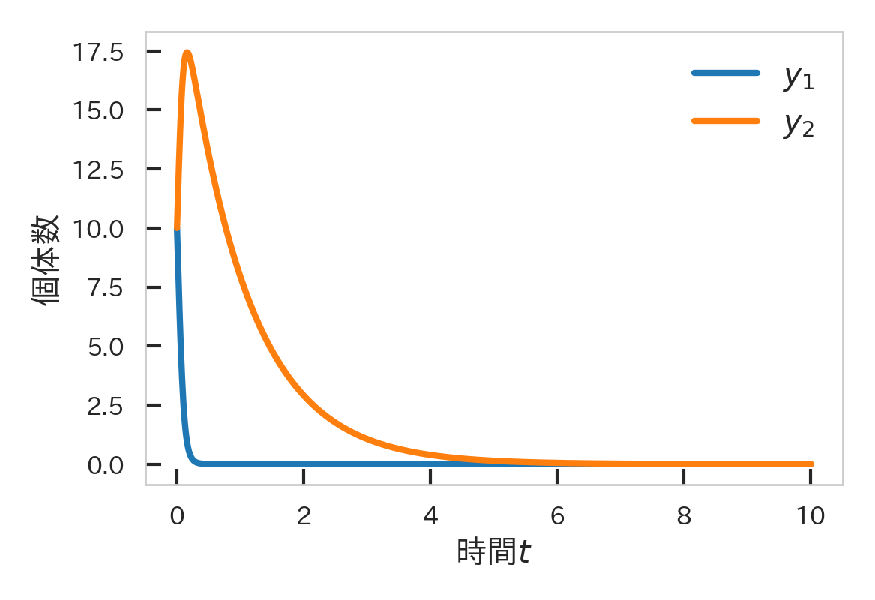
\includegraphics[scale=0.5]{ex1-1.eps}
           \end{center}
           \subcaption{実験1-1}
           \label{ex611}
          \end{minipage}

          \begin{minipage}{0.5\hsize}
           \begin{center}
            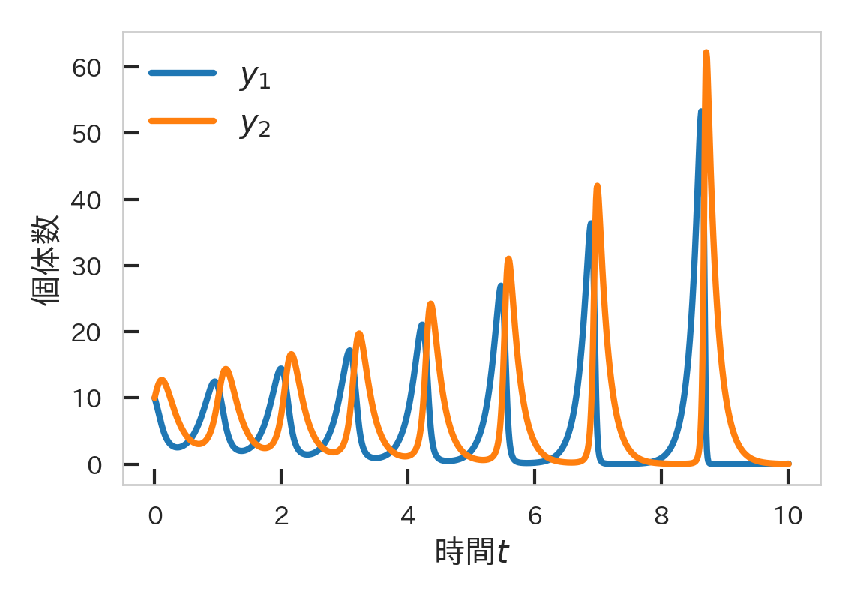
\includegraphics[scale=0.5]{ex1-2.eps}
           \end{center}
           \subcaption{実験1-2}
           \label{ex612}
          \end{minipage}
        \end{tabular}

        \begin{tabular}{c}
          \begin{minipage}{0.5\hsize}
            \begin{center}
             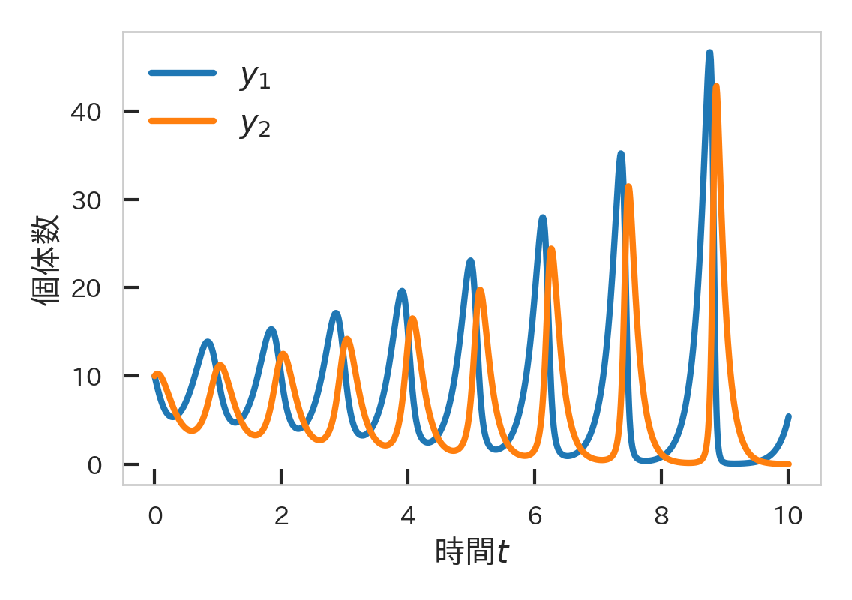
\includegraphics[scale=0.5]{ex1-3.eps}
            \end{center}
            \subcaption{実験1-3}
            \label{ex613}
           \end{minipage}

           \begin{minipage}{0.5\hsize}
            \begin{center}
             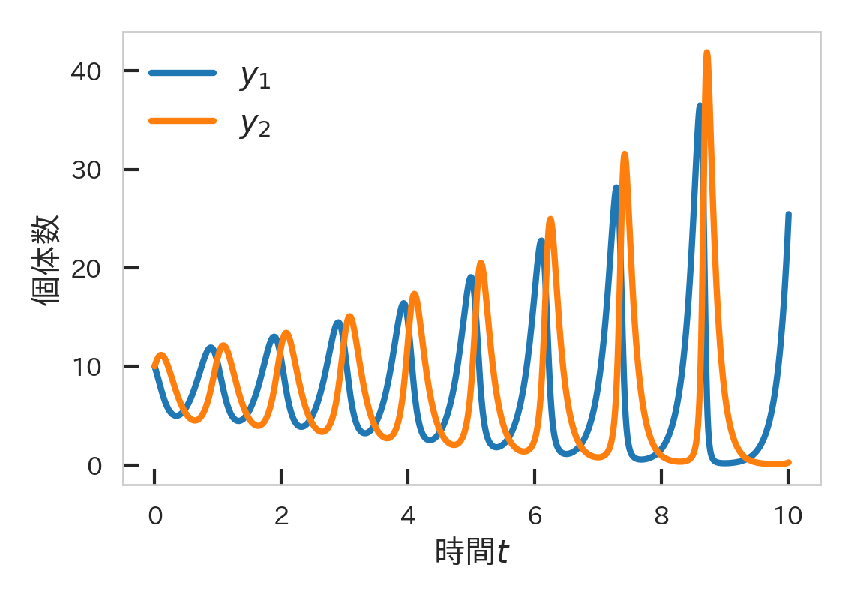
\includegraphics[scale=0.5]{ex1-4.eps}
            \end{center}
            \subcaption{実験1-4}
            \label{ex614}
           \end{minipage}
          \end{tabular}
          \caption{実験1の結果}
          \label{exp1}
         \end{figure}

         図\ref{ex611}は表\ref{result1-params}に示した実験1-1の結果をグラフにしたものである.まず,実行結果と手計算
         で求めたオイラー法の値が一致することを確認する.表\ref{result1-1acc}に実験1-1における実行結果から得られた値と
         手計算によって計算した値である.表\ref{result1-1acc}では時間$t$が0.01から0.03までの場合について,
         手計算行った.
      \begin{table}[H]
        \caption{実験結果と手計算の比較}
      \label{result1-1acc}
      \begin{center}
          \begin{tabular}{c|l l|l l}\hline
             & \multicolumn{2}{c|}{実験結果} & \multicolumn{2}{c}{手計算} \\ \cline{2-5}
             時間$t$ & \multicolumn{1}{c}{$y_1$} & \multicolumn{1}{c|}{$y_2$} & \multicolumn{1}{c}{$y_1$} & \multicolumn{1}{c}{$y_2$} \\ \cline{1-5}
             0 & 10 & 10 & 10 & 10 \\ 
0.01 & 9.1 & 10.9 & 9.1 & 10.9 \\
0.02 & 8.1991 & 11.7829 & 8.1991 & 11.7829 \\
0.03 & 7.314999 & 12.631163 & 7.314999 & 12.631163 \\ \hline
          \end{tabular}
      \end{center}
      \end{table}
      手計算の方法を例を交えて説明する.パラメータはすべて1だから,計算する連立方程式微分方程式は
      式(\ref{all1})である.式(\ref{all1})をオイラー法の計算式にすると式(\ref{all11})になる.
      \begin{eqnarray}
        \begin{cases}
          \frac{dy_1}{dx} = y_1-y_1y_2 & \\
          \frac{dy_2}{dx} = y_2+y_1y_2 &
        \end{cases}
        \label{all1}
      \end{eqnarray}

      \begin{eqnarray}
        \begin{cases}
          y_{1(i+1)} = y_{1(i)}+h(y_{1(i)} + y_{1(i)}y_{2(i)}) & \\
          y_{2(i+1)} = y_{2(i)}+h(-y_{2(i)} + y_{1(i)}y_{2(i)}) &
        \end{cases}
        \label{all11}
      \end{eqnarray}

      $h=0.01$のときの正しい実験結果は,$y_{1(0)}=y_{2(0)}=10$を式(\ref{all11})に代入すると,
      式(\ref{all12})に示すように計算できる.時間を$0.02,0.03 \dots $と変化させた場合も
      同じように計算を行えばよい.
      \begin{eqnarray}
        \begin{cases}
          y_{1(0.01)} = 10+0.01\cdot (10 + 10\cdot 10) = 9.1& \\
          y_{2(0.01)} = 10+0.01\cdot (-10 + 10\cdot 10) = 10.9&
        \end{cases}
        \label{all12}
      \end{eqnarray}
       表\ref{result1-1acc}の実験結果と手計算の結果から,時間$t$が$0.01$から$0.03$のとき,
      実行結果と手計算の結果が一致していることがわかる.時間$t$が$0.01$から$0.03$の3例で
      すべての実行結果と手計算に誤差がないとは言えないから,excelによる計算結果と実行結果
      を比較する.図\ref{gosa}にexcelによる計算と実行結果の差を示す.
      \begin{figure}[H]
        \centering
        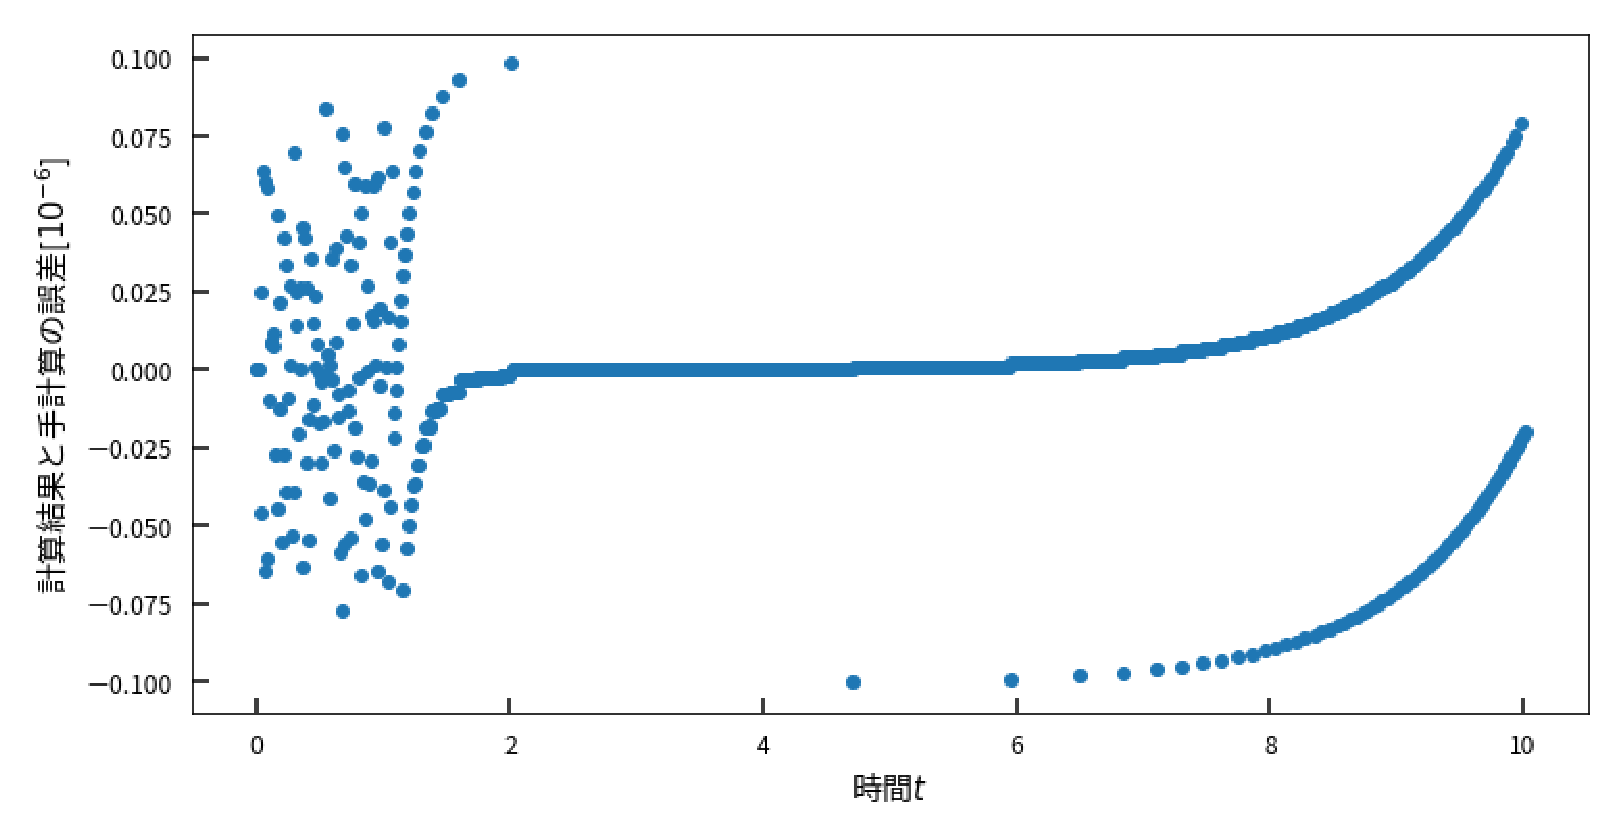
\includegraphics[scale=0.5]{ex11error.eps}
        \caption{計算結果の差}
         \label{gosa}
        \end{figure}
        
        図\ref{gosa}において,手計算と実行結果の差は$10^{-7}$程度であることがわかる.
        これより,実行結果と手計算が一致していると考えられる.よって実行結果は正しいと
        言える.\\
         実行結果が正しいことがわかったから,パラメータを変化させたときの実行結果
        について観察する.実験1の4つの実験結果に共通していることは,$y_1$,$y_2$の値
        が0以上であるということである.$y_1$は被食者,$y_2$は捕食者を表していた.
        式(\ref{rotoka})のモデルの特性は後で考察するが,$y_1$,$y_2$が
        非負であることは,モデルによる生物の個体数の増減のシミュレーションの
        結果が非常にわかりやすくなる.さらに,$a$,$b$を固定して,$c$,$d$を入れ替えた
        実験1-3,実験1-4の結果に注目する.実験1-3と実験1-4の結果は$y_1$,$y_2$が入れ替わ
        っただけである.このことから,$a$,$b$を固定したとき,$c$,$d$は対称関係にあり,
        $c$,$d$のうち,値の大きいほうが,周期的な立ち上がりが大きいことがわかる.
      

      \subsubsection{実験2の結果}
      実験2は,$y_2 < a/c$かつ$y_1 > b/d$の条件下でパラメータを変化させたときの実行結果である.実験2-1および実験2-2
      結果を図\ref{exp2}に示す.図\ref{exp2}から,実験2の条件では被食者$y_2$が周期的に大量発生し,捕食者$y_1$は20前後の
      数字であることが読み取れる.このことから,$y_2 < a/c$という条件が満たされるようなモデルは,被食者が周期的に
      大量発生し,捕食者は被食者と比較すると少数であることが考えられる.

      \begin{figure}[H]
        \begin{tabular}{c}
        \begin{minipage}{0.5\hsize}
         \begin{center}
          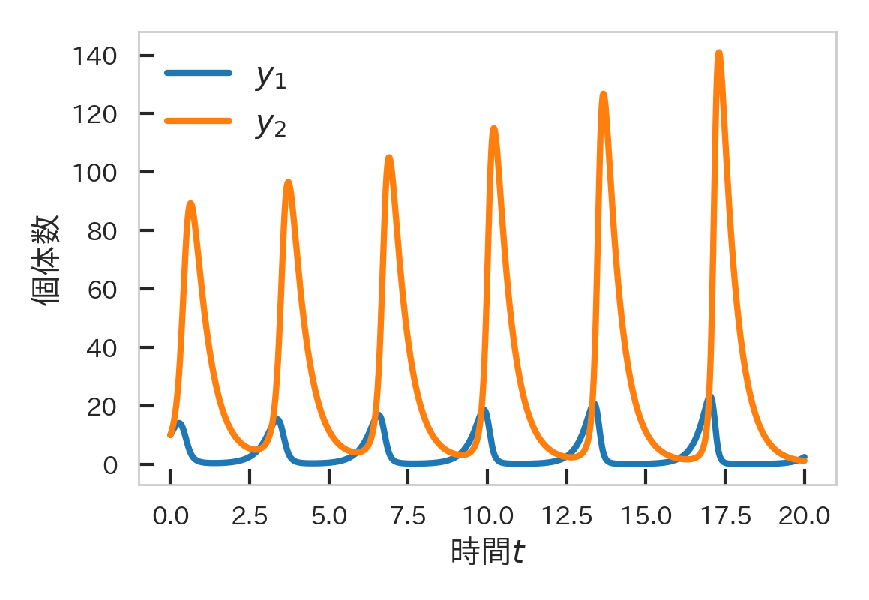
\includegraphics[scale=0.5]{ex2-1.eps}
         \end{center}
         \subcaption{実験2-1}
         \label{ex621}
        \end{minipage}

        \begin{minipage}{0.5\hsize}
         \begin{center}
          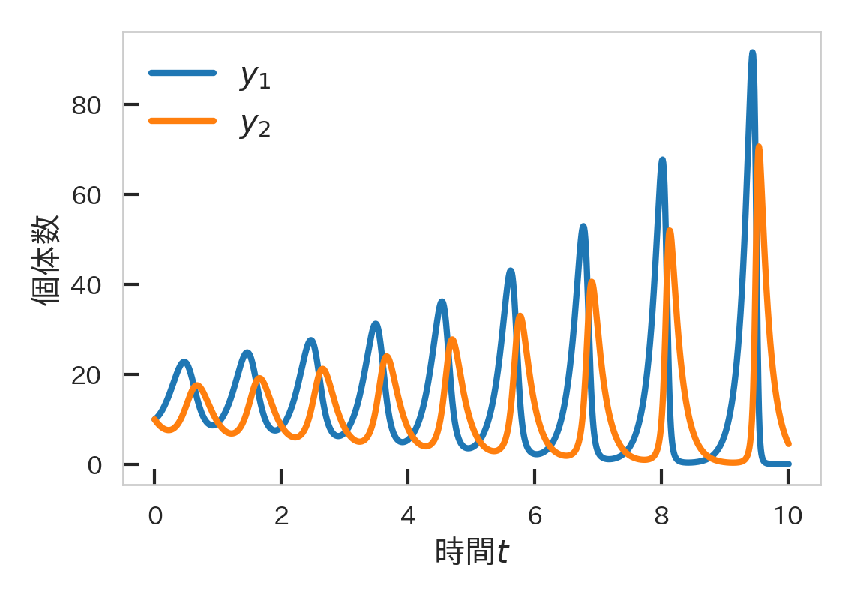
\includegraphics[scale=0.5]{ex2-2.eps}
         \end{center}
         \subcaption{実験2-2}
         \label{ex622}
        \end{minipage}
      \end{tabular}
        \caption{実験2の結果}
        \label{exp2}
       \end{figure}

      \subsubsection{実験3の結果}
      実験3は,$y_2 > a/c$かつ$y_1 < b/d$の条件下でパラメータを変化させたときの実行結果である.実験3-1および実験3-2
      結果を図\ref{exp3}に示す.図\ref{exp3}から,実験3の条件では実験2とは逆に,被食者$y_1$が周期的に大量発生し,
      捕食者$y_2$は少数であることが読み取れる.実験2および実験3から,$y_2 > a/c$または$y_1 > b/d$というどちらかの
      条件を満たすモデルでは,被食者と捕食者のバランスが悪いシミュレーション結果が得られることが考えられる.さらに,
      実験2,実験3のどちらにおいても,個体数が0に限りなく近づくタイミングがあることがわかる.今扱っているモデルでは
      連続なモデルを考えているから,個体数が0に限りなく近づいても上昇することがあるが,実際には生態系のバランス崩れた
      ことで絶滅したと考えることもできる.

      \begin{figure}[H]
        \begin{tabular}{c}
        \begin{minipage}{0.5\hsize}
         \begin{center}
          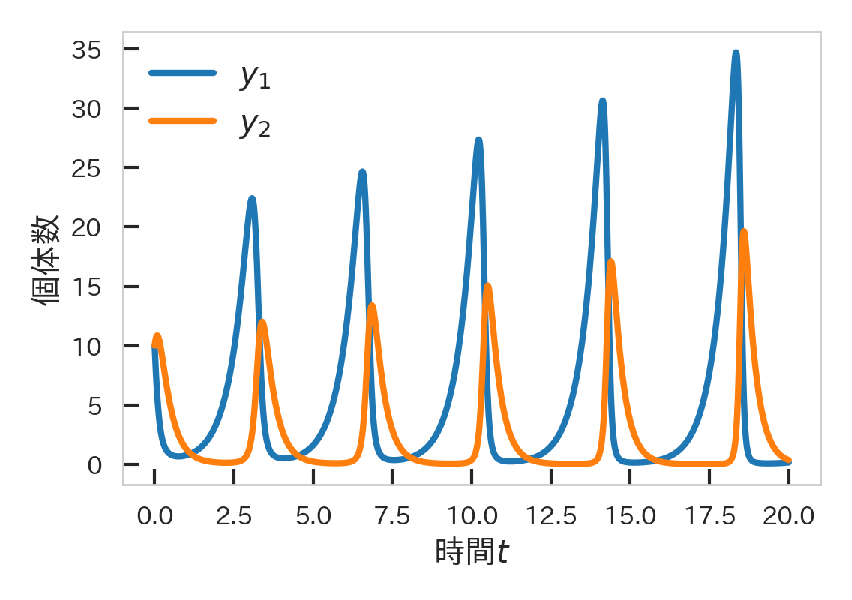
\includegraphics[scale=0.5]{ex3-1.eps}
         \end{center}
         \subcaption{実験3-1}
         \label{ex631}
        \end{minipage}

        \begin{minipage}{0.5\hsize}
         \begin{center}
          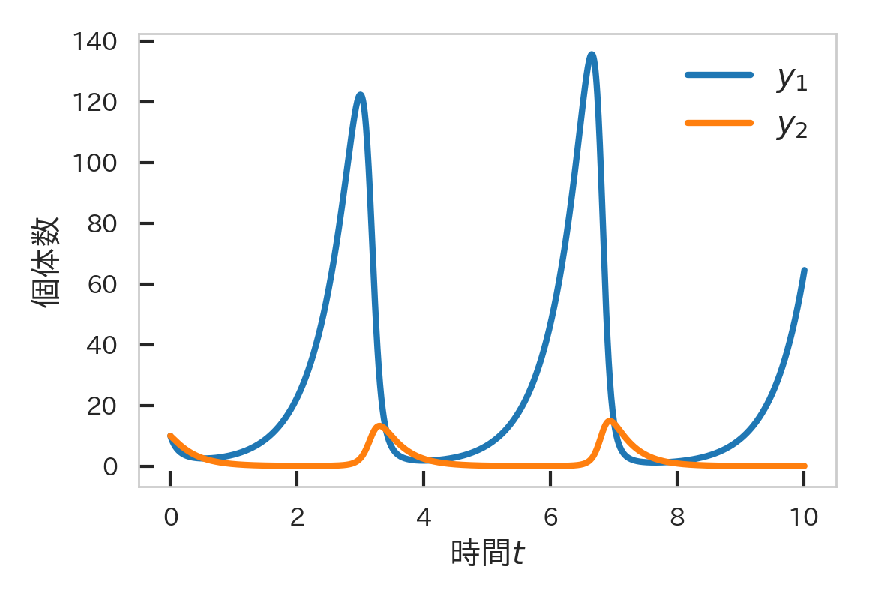
\includegraphics[scale=0.5]{ex3-2.eps}
         \end{center}
         \subcaption{実験3-2}
         \label{ex632}
        \end{minipage}
      \end{tabular}
        \caption{実験3の結果}
        \label{exp3}
       \end{figure}

      \subsubsection{実験4の結果}
      実験4は,$y_2 < a/c$かつ$y_1 < b/d$の条件下でパラメータを変化させたときの実行結果である.実験4-1から実験4-2
      までの結果を図\ref{exp4}に示す.図\ref{exp4}から実験4の結果は,パラメータによってまったく違うことが読み取れる.
      図\ref{ex641}は$y_1$,$y_2$ともに個体数が安定しており,個体数が0,つまり絶滅しにくいモデルであることが読み取れる.
      図\ref{ex642}は個体の周期的な増減に加えて,全体にトレンドがあるように見える.図\ref{ex643}は$y_1$,$y_2$の周期的な
      増加のピークの値が,増加しているモデルであるように見える.図\ref{ex644}は$t=2$で$y_1$,$y_2$ともに絶滅するモデルで
      あると読み取れる.

      \begin{figure}[H]
        \begin{tabular}{c}
        \begin{minipage}{0.5\hsize}
         \begin{center}
          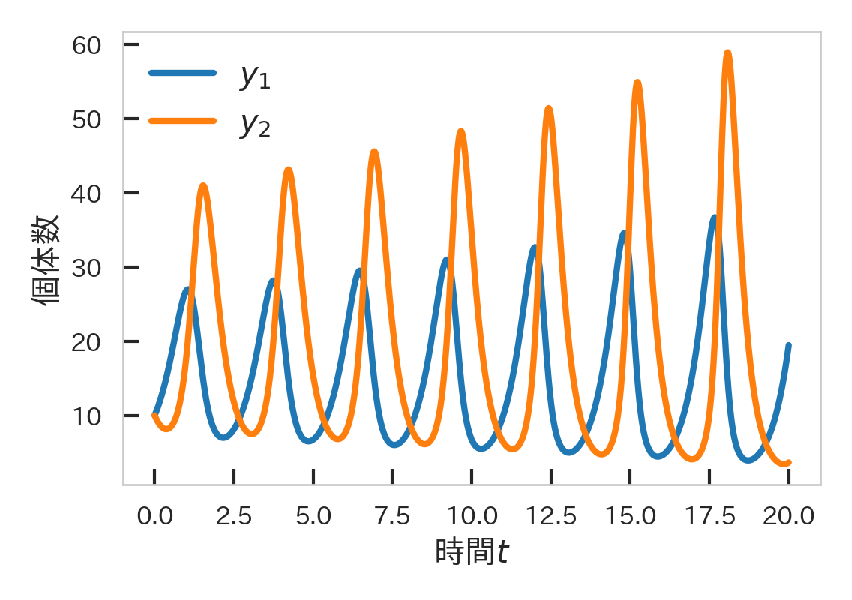
\includegraphics[scale=0.5]{ex4-1.eps}
         \end{center}
         \subcaption{実験4-1}
         \label{ex641}
        \end{minipage}

        \begin{minipage}{0.5\hsize}
         \begin{center}
          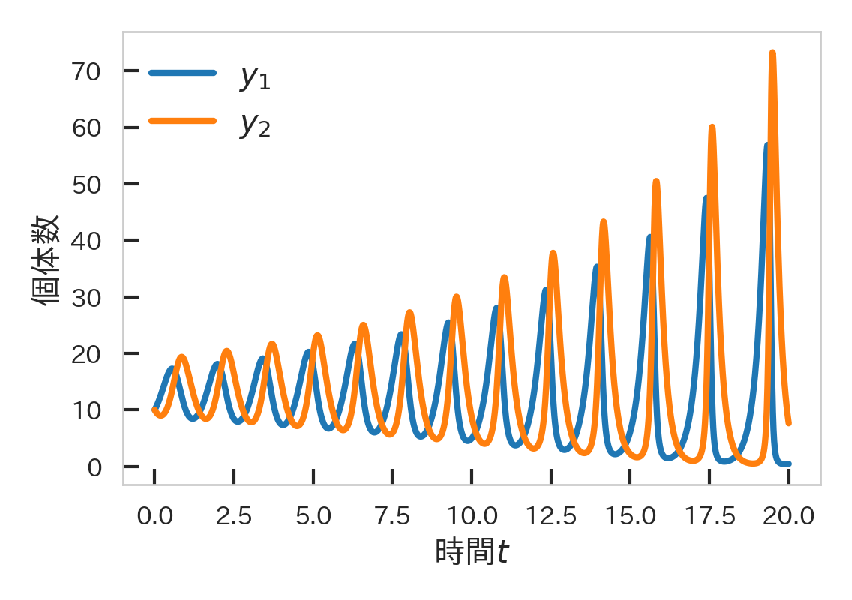
\includegraphics[scale=0.5]{ex4-2.eps}
         \end{center}
         \subcaption{実験4-2}
         \label{ex642}
        \end{minipage}
      \end{tabular}

      \begin{tabular}{c}
        \begin{minipage}{0.5\hsize}
          \begin{center}
           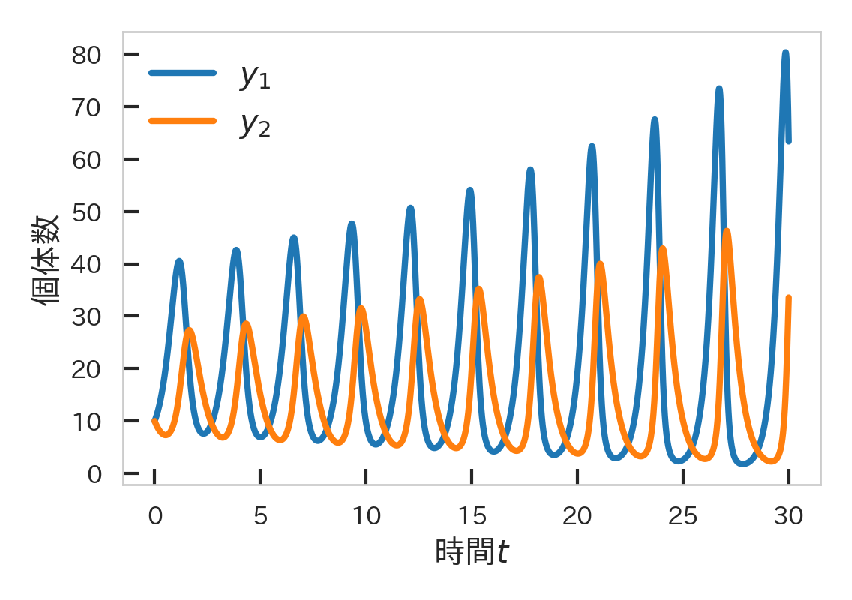
\includegraphics[scale=0.5]{ex4-3.eps}
          \end{center}
          \subcaption{実験4-3}
          \label{ex643}
         \end{minipage}

         \begin{minipage}{0.5\hsize}
          \begin{center}
           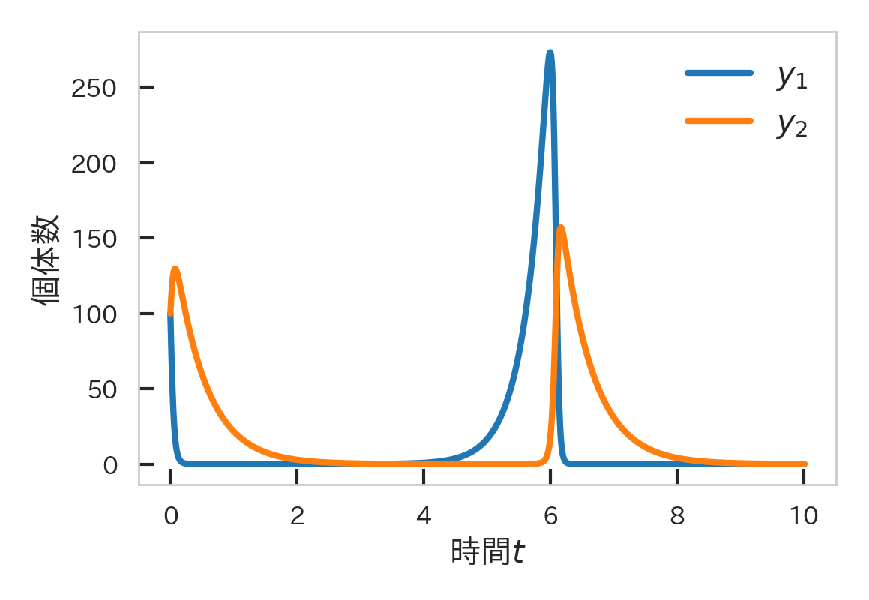
\includegraphics[scale=0.5]{ex4-4.eps}
          \end{center}
          \subcaption{実験4-4}
          \label{ex644}
         \end{minipage}
        \end{tabular}
        \caption{実験4の結果}
        \label{exp4}
       \end{figure}

      \subsection{考察}
       実験1~4の結果から,パラメータa,b,c,dの意味を考察する.式(\ref{rotoka})からパラメータaは
       被食者の繁殖のしやすさ,パラメータbは捕食者の減少のしやすさを意味すると考えられる.パラメータcは
       実験2から捕食者の数に比例した被食者の減少のしやすさであると考えられる.パラメータdは実験3から
       被食者の数に比例した捕食者の繁殖のしやすさであると考える.
       

      \section{課題7}
      本章では課題7における,課題内容,プログラムの説明,実行結果の3つについて述べる.
      \subsection{課題内容}
      課題7では,ばね定数$k$のばねに質量$m$の物体がつながっているときの単振動のシミュレーションを行う.
      本課題では床との摩擦を考慮し,摩擦係数の大きさ$l$とする.
      このときの運動方程式は式(\ref{soe})のように書ける.初期条件は$y(0)=10,y'(0)=0$とする.高階微分方程式をそのまま数値計算を行うことは
      できない.我々が扱えるのは,連立微分方程式であるから,これに帰着するように式変形を行う.
      \begin{equation}
        \frac{d^2x}{dt^2}+\frac{k}{m}x=-lv
        \label{soe}
      \end{equation}
      $v=\frac{dx}{dt}$とおくと,式(\ref{soe})は式(\ref{bane})で表せる.また,式(\ref{bane})のときの初期条件は,$y(0)=10,v(0)=0$となる.
      式(\ref{bane})は連立方程式微分方程式であるから,課題6のプログラムを改変すれば数値計算を行うことができる.
      \begin{eqnarray}
        \begin{cases}
          v = \frac{dx}{dt} & \\
          \frac{dv}{dt} = -kx-lv &
        \end{cases}
        \label{bane}
      \end{eqnarray}


      \subsection{プログラムの説明}
      課題7のプログラムは,課題6のプログラムのメイン関数を改変しただけである.リスト\ref{main7}にメイン関数のコードを示す.
      リスト\ref{main7}において,質量$m$は変数m,ばね定数$k$は変数k,摩擦係数は$l$は変数lで管理している.
      \begin{lstlisting}[basicstyle=\ttfamily\footnotesize, frame=single,label=main7,caption=メイン関数のコード]
int main(void){
    double h = 0.01;
    double lim=10.0;
    double m=1;
    double k=2;
    double l=0;
    double step;
    int i;
    double initVector[DIM][1] ={{10},{0}}; // 初期条件 y,v 
    double transVector[DIM+1][1];
    double weightMatrix[DIM][DIM+1] = {{0,0,1},
                                        {0,-k/m,-l/m}
                                       };
    double yiVector[DIM][1];
    double tmpVector[DIM][1];
    double resultVector[DIM][1];

    setVector(initVector,yiVector);
    for(step=h;step<=lim;step+=h){
        transformVector(yiVector,transVector);
        multipleMatrix(weightMatrix,transVector,tmpVector);
        scalerVector(tmpVector,h);
        addVector(yiVector,tmpVector,resultVector);
#ifdef STDOUT
        printf("step = %lf\n",step);
        printf("y = %lf\n",resultVector[0][0]);
        printf("v = %lf\n",resultVector[1][0]);
        printf("\n");
#else
        printf("%lf,%lf,%lf\n",step,resultVector[0][0],resultVector[1][0]);
#endif
        setVector(resultVector,yiVector);
    }
    return 0;
}
            \end{lstlisting}     

      \subsection{実行結果}
      実行結果として,次の2つを確認する.
      \begin{enumerate}
        \item $l=0$のとき単振動になることの確認
        \item $l,k$の値を変更した場合の動作
      \end{enumerate}  

      \subsubsection{$l=0$のときの実行結果}
      $l=0$のとき,単振動になることを確認する. $l=0$のとき,式(\ref{soe})は式(\ref{tansindo1})のように書き直せる.
      さらに,角速度$\omega(\omega >0)$を用いると式(\ref{tansindo1})は式(\ref{tansindo2})のように表せる.これより, $\omega=\sqrt{\frac{k}{m}}$という関係が
      あることがわかる.一方で,周期$T$と角速度$\omega$には式(\ref{shuki})に示す関係がある. これらより,
      周期$T$は式(\ref{shukikm})に,示すようにばね定数$k$および質量$m$で表すことができる.

      \begin{eqnarray}
        \frac{d^2x}{dt^2} &=& -\frac{k}{m}x \label{tansindo1} \\
        &=& -\omega^2 x \label{tansindo2} 
      \end{eqnarray}

      \begin{eqnarray}
        T &=& \frac{2 \pi }{\omega} \label{shuki} \\
         &=& 2\pi \sqrt{\frac{m}{k}} \label{shukikm}
      \end{eqnarray}

      さらに,式(\ref{tansindo2})の微分方程式は簡単に解を求めることができる.解を求める方法については省略するが,式(\ref{tansindo2})を
      解くと式(\ref{tansindo3})の一般解が得られる($C_1,C_2$は任意定数).初期条件および$m=1$という指定を式(\ref{tansindo3})に
      代入すると, $l=0$のときの位置$x$は式(\ref{tansindo4})で表せる.さらに,式(\ref{tansindo4})から速度$v$は式(\ref{tansindo5})
      で表せる.
      \begin{eqnarray}
        x &=& C_1 \sin(\omega t) + C_2 \cos(\omega t) \label{tansindo3} \\
        x &=& 10\cos(\sqrt{k} t) \label{tansindo4} \\
        v &=& -10\sqrt{k} \sin(\sqrt{k} t) \label{tansindo5}
      \end{eqnarray}

      式(\ref{tansindo4})は振幅が10の余弦関数であり,式(\ref{tansindo5})は振幅10の正弦関数である.これより,シミュレーションの結果は位置$y$が振幅が10の余弦関数,
      速度$v$が振幅が10の制限関数になることを確認すればよい.
      図\ref{l0k2m1}~図\ref{l0k4m1v}にシミュレーションの結果を示す.図\ref{l0k2m1}は$l=0$,$k=2$のときの位置$y$,図\ref{l0k4m1}は$l=0$,$k=4$のとき位置$y$
      のグラフである.図\ref{l0k2m1v}は$l=0$,$k=2$のときの速度$v$,図\ref{l0k4m1v}は$l=0$,$k=4$のとき速度$v$
      のグラフである.図\ref{l0k2m1}および図\ref{l0k4m1}から,シミュレーションの結果はおおよそ余弦関数の理論値と一致していることが読み取れる.
      図\ref{l0k2m1v}および図\ref{l0k4m1v}についても,シミュレーションの結果はおおよそ正弦関数の理論値と一致していることが読み取れる.
      これらより,$l=0$のとき単振動になることが確認できた.

      \begin{figure}[H]
      \centering
      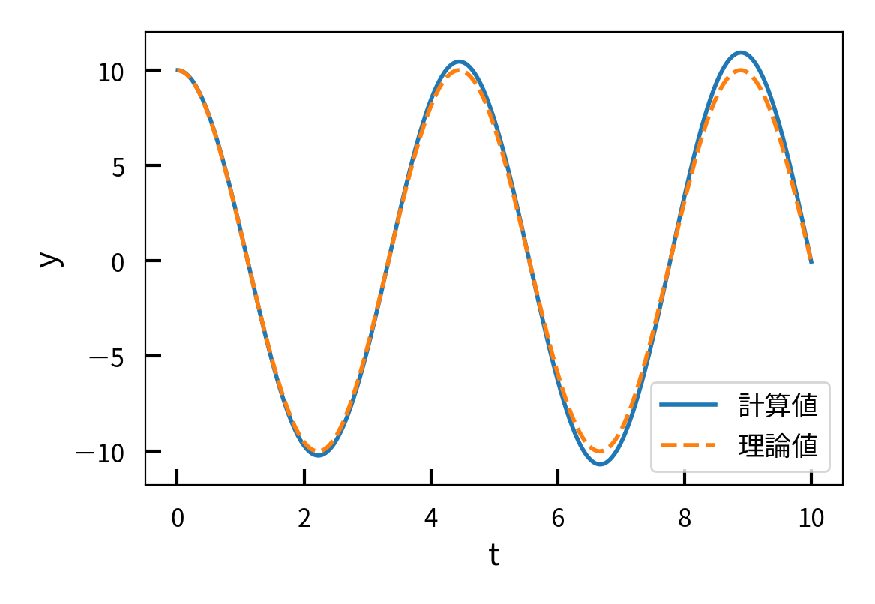
\includegraphics[scale=0.6]{l0k2.eps}
      \caption{$l=0$,$k=2$のときの実行結果($y$)}
      \label{l0k2m1}
      \end{figure}

      \begin{figure}[H]
        \centering
        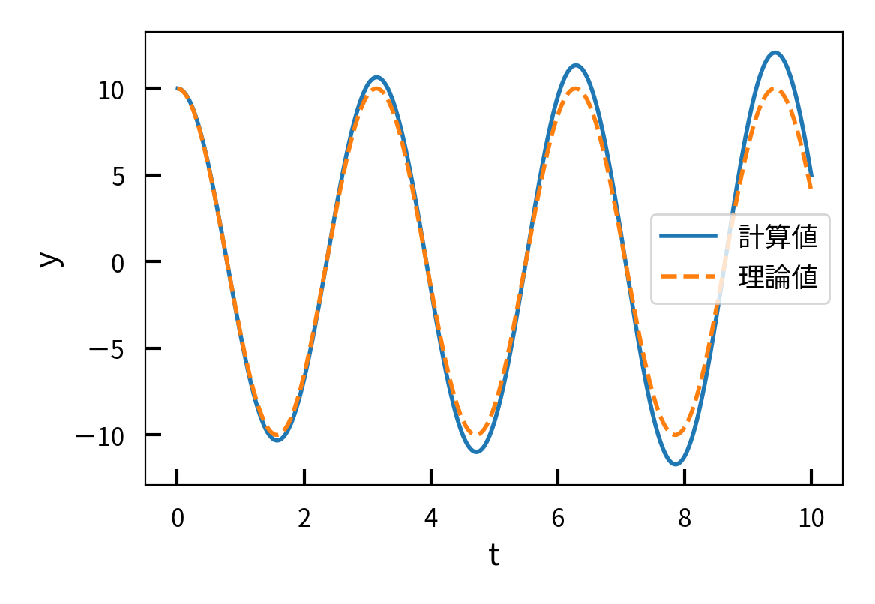
\includegraphics[scale=0.6]{l0k4.eps}
        \caption{$l=0$,$k=4$のときの実行結果($y$)}
        \label{l0k4m1}
        \end{figure}

      \begin{figure}[H]
      \centering
      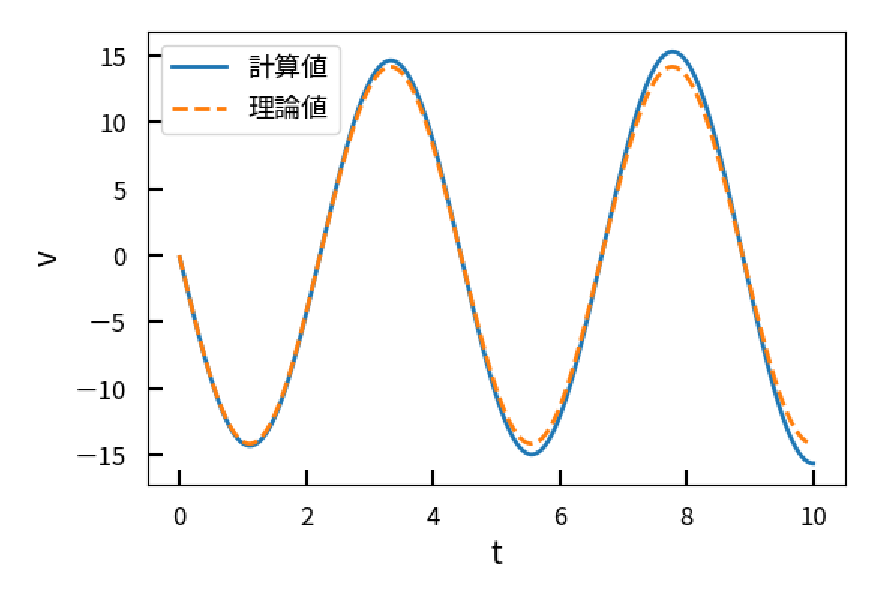
\includegraphics[scale=0.6]{l0k2v.eps}
      \caption{$l=0$,$k=2$のときの実行結果($v$)}
      \label{l0k2m1v}
      \end{figure}

      \begin{figure}[H]
        \centering
        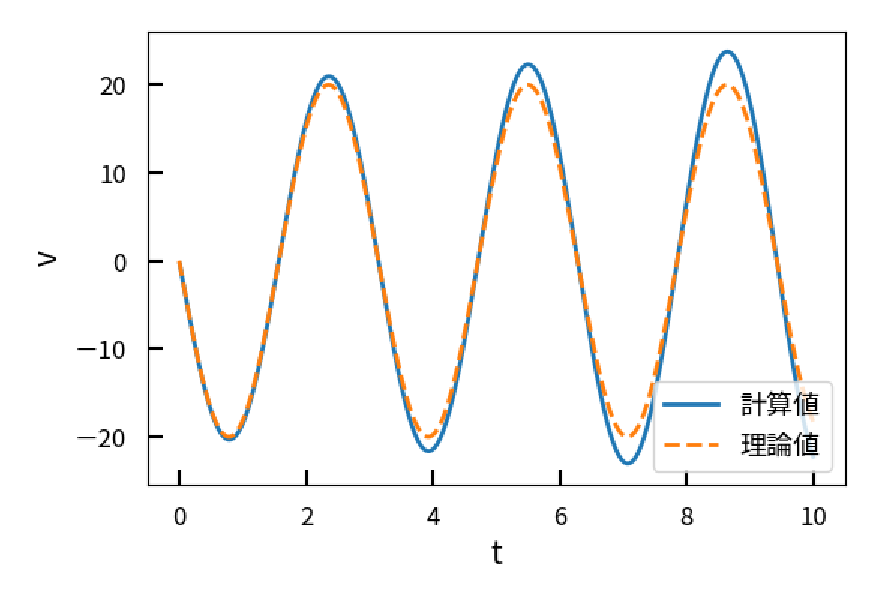
\includegraphics[scale=0.6]{l0k4v.eps}
        \caption{$l=0$,$k=4$のときの実行結果($v$)}
        \label{l0k4m1v}
        \end{figure}
    

        次に$l,k$の値を変更した場合の動作について確認する. 刻み幅は次節の考察で述べるように,時間によらず振幅が一定になるような刻み幅$h=0.001$を用いる.
        図\ref{l1k2}および図\ref{l3k2}に$l$を変化させたときの実行結果を示す.図\ref{l1k2}は$l=1$,図\ref{l3k2}は$l=3$のときの実行結果である.
        図\ref{l1k2}および図\ref{l3k2}から摩擦力の項があると,振動が徐々に減衰して静止する運動になることがわかる.単振動に摩擦力があると,これは徐々に
        振動が弱くなり,最終的には停止するというイメージに一致する.
        
        \begin{figure}[H]
          \centering
          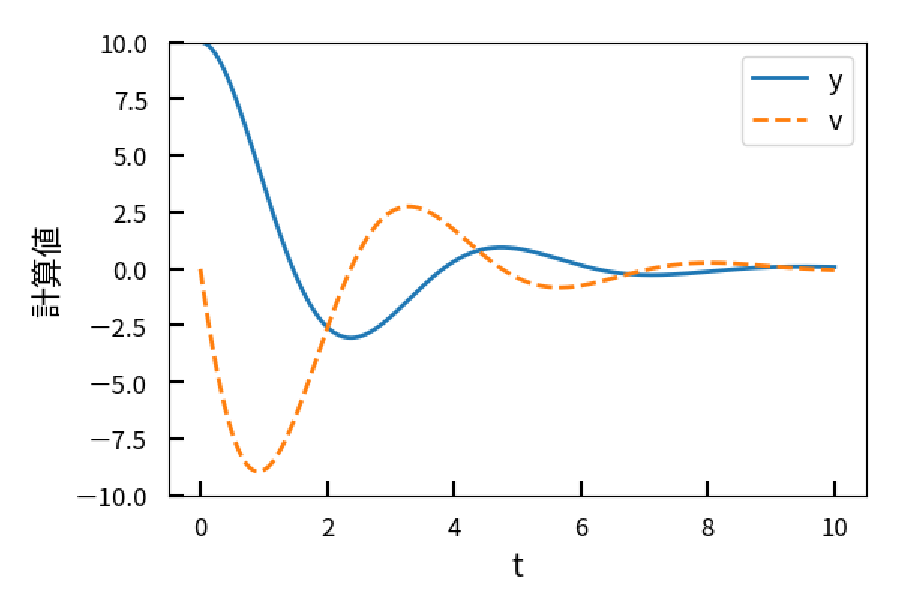
\includegraphics[scale=0.6]{l1k2.eps}
          \caption{$l=1$,$k=2$のときの実行結果}
          \label{l1k2}
          \end{figure}

      \begin{figure}[H]
      \centering
      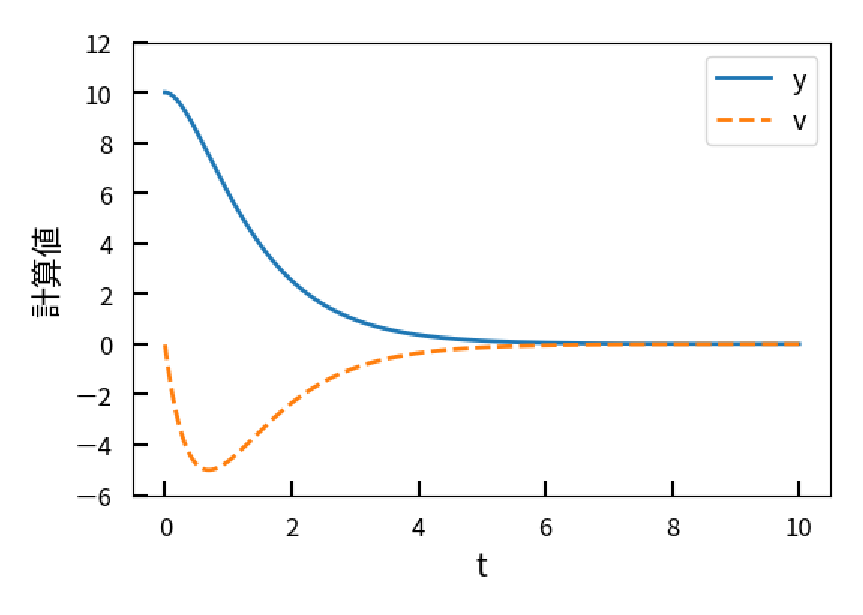
\includegraphics[scale=0.6]{l3k2.eps}
      \caption{$l=3$,$k=2$のときの実行結果}
      \label{l3k2}
      \end{figure}

      \subsection{考察}
      図\ref{l0k2m1}および図\ref{l0k4m1}からは,時間が経過すると誤差が大きくなってしまう特徴が読み取れる.時間によらず振幅が一定になるような刻み幅を考察する.
      ここでは$k=4$,$l=0$での3周期分の「計算値の絶対値」と「理論値の絶対値」の標準偏差を比較し,相対誤差が1\%未満になる場合の刻み幅を,振幅が一定になるような刻み幅とする.このような指標を
      設ける理由は,グラフからの視覚的な誤差の判断では,グラフの拡大縮小によって誤差の見方が変化してしまうためである.振幅が10の余弦関数を2$n$周期($n$:整数)とったときの
      標準偏差はおおよそ$\sqrt{10}=3.16$になるはずである.表\ref{h7}に刻み幅$h$を変化させて実験を行った結果を示す.表\ref{h7}から,誤差は刻み幅$h$の値を小さくすると減少し,
      $h=0.001$のとき,指標となる1\%未満になることがわかる. $h=0.001$のときの振動の様子を図\ref{h0001}に示す.図\ref{h0001}から$h=0.001$のとき,
      目視では理論値と計算値の違いがわからないほど,計算値と理論値の誤差が少ないことが読み取れる.これらより$h=0.001$が振幅が一定になるような刻み幅であると
      考える.

      \begin{table}[H]
      \caption{刻み幅と誤差の関係}
      \label{h7}
      \begin{center}
      \begin{tabular}{r|c|c|c}\hline
        刻み幅 & 計算値の標準偏差 & 理論値の標準偏差 & 相対誤差[\%] \\ \hline \hline 
        0.1 & 13.71 & 3.09 & 77.46 \\
        0.05 & 6.00 & 3.08 & 94.81 \\
        0.01 & 3.62 & 3.08 & 17.53 \\
        0.005 & 3.23 & 3.08 & 4.87 \\
        0.001 & 3.11 & 3.08 & 0.97\\ \hline
      \end{tabular}
      \end{center}
      \end{table}

      \begin{figure}[H]
      \centering
      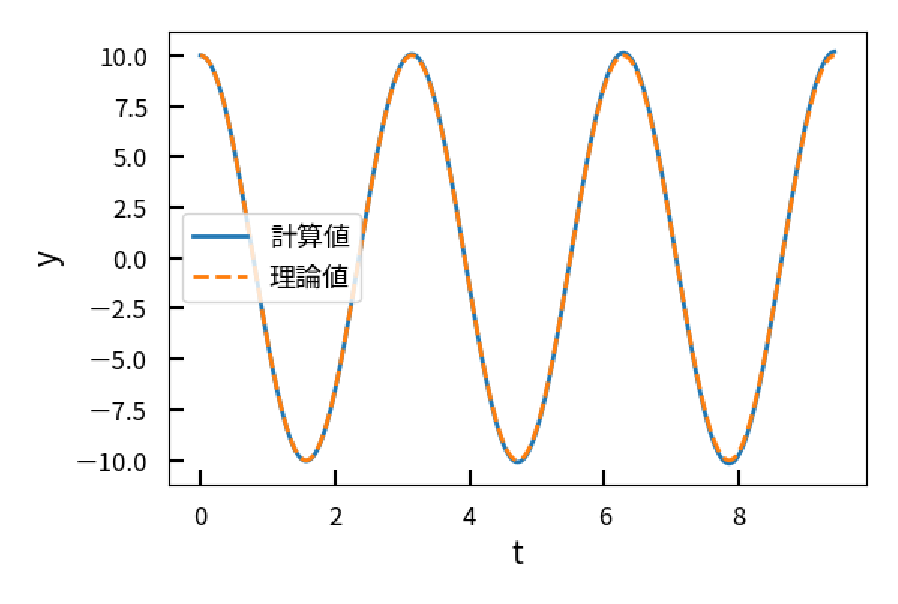
\includegraphics[scale=0.6]{h0001.eps}
      \caption{$h=0.001$のときの振動の様子}
      \label{h0001}
      \end{figure}

      \section{課題8}
      本章では課題8における,課題内容,プログラムの説明,実行結果の3つについて述べる.
      \subsection{課題内容}
      課題8では直列RLC回路の微分方程式をホイン法で解くシミュレーションを行う. ホイン法の説明は前回の第一回のレポートで行ったため省略する.
      本課題で解く微分方程式を式(\ref{RLC})に示す.初期条件は,$Q(0)=Q_0$,$\frac{d}{dt}Q(0)=0$とする.

      \begin{equation}
        L \frac{d^2Q(t)}{dt^2}+R \frac{dQ(t)}{dt}+\frac{Q(t)}{C}=0
        \label{RLC}
      \end{equation}

      式(\ref{RLC})はパラメータ$R$(レジスタンス),$L$(インダクタンス),$C$(キャパシタンス)が特殊な値のときのみ解を求めることができるが,
      一般に解を求めることができない.このためシミュレーションを行う.シミュレーションを行う場合,式(\ref{RLC})は2階微分方程式であるため
      課題7で行ったように式変形を行って連立微分方程式に帰着させる必要がある.この変形について説明する. $\frac{dQ(t)}{dt}$は物理学的には
      電流$I$を表しているから,$I(t)=\frac{dQ(t)}{dt}$とおくと,式(\ref{RLC})は式(\ref{IRLC})で表せる.初期条件も$I$を用いて
      $Q(0)=Q_0$,$I(0)=0$と書き直せる.式(\ref{RLC})から式(\ref{IRLC})の変形で2階微分方程式を連立微分方程式に帰着させることができたから,
      シミュレーションを行うことができる.

      \begin{eqnarray}
        \begin{cases}
          \frac{d I(t)}{dt}+\frac{R}{L}I(t)+\frac{Q(t)}{CL}=0 & \\
          I(t)=\frac{dQ(t)}{dt} &
        \end{cases}
        \label{IRLC}
      \end{eqnarray}


      \subsection{プログラムの説明}
      プログラムの説明を行う.リスト\ref{kadai8}にホイン法で連立微分方程式を解くプログラムを示す.
      $n$次元の連立微分方程式をホイン法で解くプログラムを作成することは難しかったため,2次の連立微分方程式を
      解くプログラムを作成した.微分方程式のパラメータ$R$,$L$,$C$および初期条件$Q_0$,$I_0$は定数として定義している.
      また,連立方程式は16行目から20行目に示す関数の形で定義している.ホイン法による連立微分方程式の計算は
      24行目から48行目に示すHeun関数で行っている.
      \begin{lstlisting}[basicstyle=\ttfamily\footnotesize, frame=single,label=kadai8,caption=課題8のプログラム]
#include<stdio.h>
#include<stdlib.h>

//define STDOUT
#define CSVOUT

#define R 0.0
#define L 10.0
#define C 0.3
#define Q0 10.0
#define I0 0.0

#define H 0.01
#define MAX_STEP 3000

double fI(double Q,double I){
    return -(R/L)*I-Q/(C*L);
}

double fQ(double I){
    return I;
}

void Heun(){
    double t = 0;
    double tp;
    double Qp,Ip,k1,k2;
    double Q=Q0;
    double I=I0;
    for(int i=0;i<MAX_STEP;i++){
        tp = t+H;
        k1 = H*fI(Q,I);
        k2 = H*fI(Q+H,I+k1);
        Ip = I+(k1+k2)/2;

        k1 = H*fQ(I);
        k2 = H*fQ(I+k1);
        Qp = Q+(k1+k2)/2;
        #ifdef STDOUT
            printf("t=%lf  Q=%0.10lf,I=%0.10lf\n",tp,Qp,Ip);
        #else
            printf("%lf,%lf,%lf\n",tp,Qp,Ip);
        #endif
        t=tp;
        I=Ip;
        Q=Qp;
    }
}

int main(int argc,char *argv[]){
    #ifdef STDOUT
        printf("t=%3d  Q=%0.10lf,I=%0.10lf\n",0,Q0,I0);
    #else
        printf("%d,%lf,%lf\n",0,Q0,I0);
    #endif    
    Heun();
    
    return 0;
}
      \end{lstlisting}

      \subsection{実行結果と考察}
      実行結果として,次に示す2つを確認する.
      \begin{enumerate}
        \item $R=0$のとき,単振動になることを確認する.また,正しく計算できる刻み幅を考察する.
        \item $R=2\sqrt{\frac{L}{C}}$付近での動作を確認する.
      \end{enumerate}
        
        まず,$R=0$のときに単振動になることを確認する. $R=0$のとき式(\ref{RLC})は式\ref{LC}となる.
        これは課題7の式(\ref{tansindo1})と同じ形の式である.これよりシミュレーションの結果は
        $Q(t)$が余弦関数,$I(t)$が正弦関数になるはずである.
        
        \begin{equation}
          \frac{d^2Q(t)}{dt^2} =-\frac{Q(t)}{LC}
          \label{LC}
        \end{equation}

        図\ref{r0}に$R=0,L=10,C=0.3$のときの実行結果を示す.刻み幅は$h=0.01$としている.
        図\ref{r0}から,$Q(t)$は振幅10の余弦関数,$I(t)$は正弦関数になっていることがわかる.
        これらより,$R=0$のときに単振動になることが確認できた.
        
        \begin{figure}[H]
          \centering
          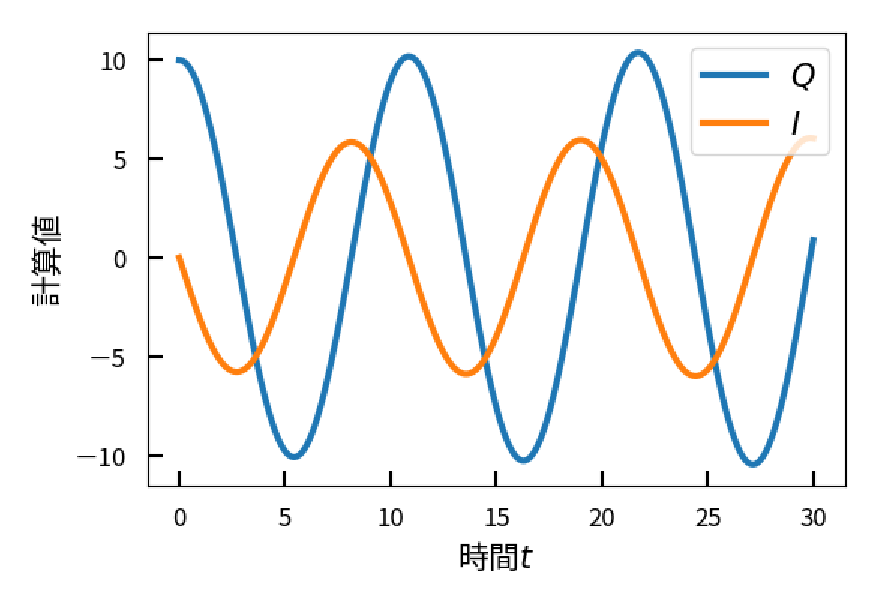
\includegraphics[scale=0.6]{r0.eps}
          \caption{$R=0$のときの実行結果}
          \label{r0}
          \end{figure}

        次に,正しく計算できる刻み幅について考察する.正しく計算できているかは課題7と同じ指標を用いて
        行う.表\ref{h8}に各刻み幅における計算値,理論値の相対誤差を示す.課題7と同様に理論値は$\sqrt{10}$
        になる.表\ref{h8}から刻み幅$h=0.001$のときに,指標となる1\%未満になっていることがわかる.このことから
        正しく計算できる刻み幅は0.001であると考察する.
        \begin{table}[H]
          \caption{刻み幅と誤差の関係}
          \label{h8}
          \begin{center}
          \begin{tabular}{r|c|c|c}\hline
            刻み幅 & 計算値の標準偏差 & 理論値の標準偏差 & 相対誤差[\%] \\ \hline \hline 
            0.1 & 4.55 & 3.08 & 47.73 \\
            0.05 & 3.64 & 3.08 & 18.18 \\
            0.01 & 3.17 & 3.08 & 2.92 \\
            0.005 & 3.12 & 3.08 & 1.30 \\
            0.001 & 3.09 & 3.08 & 0.32 \\ \hline
          \end{tabular}
          \end{center}
          \end{table}

        $R=2\sqrt{\frac{L}{C}}$付近での動作を確認する. $L=10$,$C=0.3$という条件から$R=11.54$で
        シミュレーションを行ってみる.図\ref{kado}に$R=11.54$のときの実行結果を示す.図\ref{kado}から
        $Q$,$I$どちらも,振動することなく減衰し,10秒付近で0になっていることが読み取れる.

        \begin{figure}[H]
          \centering
          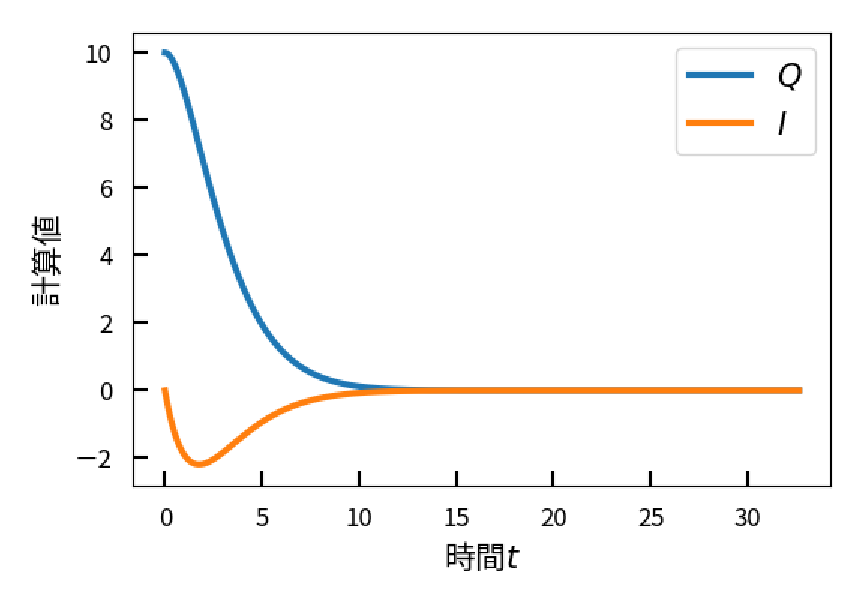
\includegraphics[scale=0.6]{kado.eps}
          \caption{$R=2\sqrt{\frac{L}{C}}$付近での実行結果}
          \label{kado}
          \end{figure}

        $R=2\sqrt{\frac{L}{C}}$付近での動作について考察する.式(\ref{RLC})の特性方程式は
        式(\ref{RLClamda})で表せる.ここで,式(\ref{RLClamda})の判別式$D$(式(\ref{D}))を考える.

        \begin{equation}
          L \lambda^2 +R \lambda + \frac{1}{C}=0
          \label{RLClamda}
        \end{equation}

        \begin{eqnarray}
          D = R^2 -4\frac{L}{C} \label{D} 
        \end{eqnarray}

        回路の動作は図\ref{r0}のように定常な場合と,図\ref{kado}のように電流,電圧が時間的に変化する2つ
        の場合に分けられる. 回路は電源投入時や切断の直後に図\ref{kado}のような動作をし,十分な時間が経過すると
        図\ref{r0}のように変化が落ち着いた状態になる.「例題と演習で学ぶ 続・電気回路」\cite{cu}によれば,
        電源投入時や切断の直後に電流,電圧が変化する状態を過度状態という.またこの現象を過度現象という.
        過度現象は判別式$D$(式(\ref{D}))の符号によって変化し,それぞれの現象には次に示すように名前がつけられている.
        \begin{itemize}
          \item $D>0$ $\dots$ 過制動
          \item $D=0$ $\dots$ 臨界制動
          \item $D<0$ $\dots$ 減衰振動
        \end{itemize}

        いま考えている現象は$R=2\sqrt{\frac{L}{C}}$という条件を,式(\ref{D})に代入すると$D=0$になることから
        臨界制動であることがわかる.臨界制動のとき式(\ref{RLC})は解くことができる.式(\ref{RLC})を解くために,
        式(\ref{RLClamda})を用いる.式(\ref{RLClamda})に$R=2\sqrt{\frac{L}{C}}$を代入して変形すると式(\ref{CL})
        のようになる.式(\ref{CL})の$CL$を式(\ref{alpha})に示すように$\alpha$とおく.
        \begin{eqnarray}
          CL \lambda^2 +2\sqrt{CL} \lambda + 1=0 \label{CL} \\ 
          \alpha \lambda^2 +2\sqrt{\alpha} \lambda + 1=0 \label{alpha}
        \end{eqnarray}

        判別式$D=0$より,$\lambda$が2重解を持つことがわかるから,式(\ref{alpha})を式(\ref{hyojun})に示すように,
        標準系に変形する.式(\ref{hyojun})から,式(\ref{lmd})に示すように$\lambda$を求められる.これより臨界制動のときの
        $Q(t)$の一般解は式(\ref{qgeneral})で表せる.$C_1,C_2$は任意定数である.
        \begin{eqnarray}
          (\sqrt{\alpha} \lambda +1)^2 &=& 0 \label{hyojun} \\ 
          \lambda &=& -\frac{1}{\sqrt{\alpha}} \label{lmd} \\
          Q(t) &=& (C_1+C_2 t)e^{-\frac{1}{\sqrt{\alpha}}t} \\
          Q(t) &=& (C_1+C_2 t)e^{-\frac{1}{\sqrt{CL}}t} \label{qgeneral} 
        \end{eqnarray}

        初期条件$Q(0)=10,I(0)=0$から,$Q(t),I(t)$の特殊解を計算する.
        式(\ref{qgeneral})から$Q(0)$を計算すると式(\ref{c1})に示すように$C_1=10$であることがわかる.
        \begin{eqnarray}
          Q(0) = C_1 = 10 \label{c1}
        \end{eqnarray}

        $C_2$は$Q(t)$の微分,つまり$I(t)$に初期条件を代入することで求めることができる.
        $I(t)$を実際に計算すると式(\ref{it})のようになる.式(\ref{it})に初期条件を代入すると,
        式(\ref{c2})に示すように$C_2=\frac{10}{\sqrt{CL}}$であることがわかる.
        \begin{eqnarray}
          I(t) &=& \frac{dQ}{dt} \\
               &=& C_2e^{-\frac{1}{\sqrt{CL}}t} -\frac{1}{\sqrt{CL}}(C_1+C_2 t)e^{-\frac{1}{\sqrt{CL}}t} \label{it} \\
          I(0) &=& C_2 -\frac{1}{\sqrt{CL}}C_1 = 0 \\
              C_2 &=& \frac{10}{\sqrt{CL}} \label{c2}
        \end{eqnarray}

        これらより, $Q(t)$の特殊解は式(\ref{qs}), $I(t)$の特殊解は式(\ref{is})に示すようになる.
        \begin{eqnarray}
          Q(t) &=& 10(1+\frac{t}{CL})e^{-\frac{1}{\sqrt{CL}}t} \label{qs} \\
          I(t) &=& -\frac{10}{CL}t e^{-\frac{1}{\sqrt{CL}}t} \label{is} 
        \end{eqnarray}        

        図\ref{kado}から,式(\ref{qs})および式(\ref{is})は,時間$t$を大きくすると0に収束するという特徴が
        あることが考えられる.このことは,式(\ref{qs})および式(\ref{is})の本質部分である$e^{-t}$および$te^{-t}$の無限大の
        極限をとることで確認できる.$e^{-t}$の無限大の極限は0である.式(\ref{rop})から式(\ref{ropzero})に$te^{-t}$の無限大の極限を計算した結果を示す.
        式(\ref{rop})の右辺から,分母分子がともに無限大の極限であることがわかる.このため,式(\ref{rop})から式(\ref{rop2})の
        展開にはロピタルの定理を用いてる.$te^{-t}$の無限大の極限は0になるから,図\ref{kado}のシミュレーション結果と一致していることが
        確認できた.
        \begin{eqnarray}
          \lim_{t \to \infty} te^{-t} = \lim_{t \to \infty} \frac{t}{e^t} \label{rop} \\
                                      = \lim_{t \to \infty} \frac{1}{e^t} \label{rop2} \\
                                      = 0 \label{ropzero}
        \end{eqnarray}  

        \section{課題9,課題10}
      本章では課題9および課題10における,課題内容,プログラムの説明,実行結果の3つについて述べる.
      \subsection{課題内容}
      課題9および課題10では,電場および磁場中を運動する電荷の運動のシミュレーションを行う.
      電荷$q$の速度\mbox{\boldmath $v$},電場\mbox{\boldmath $E$},磁場\mbox{\boldmath $B$}とすると電荷が受ける力\mbox{\boldmath $F$}
      は式\ref{uf}で与えられる.
      \begin{eqnarray}
        \mbox{\boldmath $F$} = q(\mbox{\boldmath $E$}+\mbox{\boldmath $v$} \times \mbox{\boldmath $B$}) \label{uf}
      \end{eqnarray}

      まず課題9では\mbox{\boldmath $E$}$=0$かつ,磁場\mbox{\boldmath $E$}$=(0,0,B_0)$の場合について考える.
      磁場\mbox{\boldmath $E$}$=(0,0,B_0)$の意味は大きさが$B_0$で成分が
      z成分のみであることを表している. \mbox{\boldmath $E$}$=0$のとき,式(\ref{uf})は
      ローレンツの法則と呼ばれ,外積を成分表示に直して計算すると式(\ref{lorentz})のようになる.
      \begin{eqnarray}
        \mbox{\boldmath $F$} &=& q+\mbox{\boldmath $v$} \times \mbox{\boldmath $B$} \\
        &=& q
        \left|
          \begin{array}{ccc}
            \mbox{\boldmath $i$} & \mbox{\boldmath $j$} & \mbox{\boldmath $k$} \\
            v_x & v_y & v_z \\
            0 & 0 & B_0 
          \end{array}
        \right| \\
        &=& q(v_y B_0,-v_x B_0,0)
      \label{lorentz}
    \end{eqnarray}

    運動方程式$m\frac{d^2}{dt^2}$\mbox{\boldmath $P$}$=$\mbox{\boldmath $F$}より式(\ref{lorentz})の左辺を書き直すと,電荷の運動は式(\ref{eqE0})
    に示すようになる.課題9では式(\ref{eqE0})のシミュレーションを行う.
    \begin{eqnarray}
      \begin{cases}
        \frac{d^2x}{dt^2} = \frac{q}{m}v_y B_0 , \frac{dx}{dt} = v_x \\
        \frac{d^2y}{dt^2} = -\frac{q}{m}v_x B_0 , \frac{dy}{dt} = v_y 
      \end{cases}
      \label{eqE0}
    \end{eqnarray}

    電場と速度は,力に垂直であるという関係がある.このため,仕事は行われず,速度の大きさは変化しない.このため,速度の大きさは式(\ref{vxvy})に示すように
    定数になる.シミュレーションの結果は刻み幅の取り方によって式(\ref{vxvy})が成り立たない場合がある.このため,式(\ref{vxvy})が成り立つ刻み幅を考察する.
    \begin{eqnarray}
      v_x ^2 + v_y ^2 = constant
      \label{vxvy}
    \end{eqnarray}

    課題10では\mbox{\boldmath $E$}$=(0,0,E_z)$($E_x$:定数)の場合の場合について考える.課題10の条件で式(\ref{uf})を成分表示すると式(\ref{ef})のようになる.
    課題10では式(\ref{ef})のシミュレーションを行う.

    \begin{eqnarray}
      \begin{cases}
        \frac{d^2x}{dt^2} = \frac{q}{m}(E_x + v_y B_0) , \frac{dx}{dt} = v_x \\
        \frac{d^2y}{dt^2} = -\frac{q}{m}(E_y - v_x B_0) , \frac{dy}{dt} = v_y \\
        \frac{d^2z}{dt^2} = \frac{q}{m}E_z , \frac{dz}{dt} = v_z
      \end{cases}
      \label{ef}
    \end{eqnarray}
    
      \subsection{プログラムの説明}
      本節では課題9および課題10のプログラムの説明について述べる.
      \subsubsection{課題9のプログラム}
    リスト\ref{kadai9}に課題9のシミュレーションを行うコードを示す.微分方程式のパラメータは定数として定義している.
    定数QBMは式(\ref{eqE0})における$\frac{q}{m}B_0$のことである.速度の計算はvelocity関数,位置の計算はdisplacement関数
    で行っている.ホイン法によるシミュレーションはHeun関数で行っている.
      \begin{lstlisting}[basicstyle=\ttfamily\footnotesize, frame=single,label=kadai9,caption=課題9のコード]
#include<stdio.h>
#include<stdlib.h>

//#define STDOUT
#define CSVOUT

#define QBM 2.0
#define X0 0.1
#define Y0 0.0
#define V0X 0.0
#define V0Y 0.1

#define H 0.001
#define MAX_STEP 10000

double velocity(double v){
    return QBM*v;
}

double displacemant(double v){
    return v;
}

void Heun(){
    double t = 0;
    double tp;
    double Xp,Yp,Vxp,Vyp,k1,k2,l1,l2;
    double x=X0;
    double vx=V0X;
    double y=Y0;
    double vy=V0Y;
    for(int i=0;i<MAX_STEP;i++){
        tp = t+H;
        k1 = H*displacemant(vx);
        l1 = H*velocity(vy);

        k2 = H*displacemant(vx+k1);
        l2 = H*velocity(vy+l1);

        Xp = x+(k1+k2)/2;
        Vxp = vx+(l1+l2)/2;

        k1 = H*displacemant(vy);
        l1 = -H*velocity(vx);

        k2 = H*displacemant(vy+k1);
        l2 = -H*velocity(vx+l1);

        Yp = y+(k1+k2)/2;
        Vyp = vy+(l1+l2)/2;

        #ifdef STDOUT
            printf("t=%lf  X =%0.10lf,Y =%0.10lf  Vx =%0.10lf,Vy =%0.10lf |v| =%lf\n"
            ,tp,Xp,Yp,Vxp,Vyp,Vxp*Vxp+Vyp*Vyp);
        #else
            printf("%lf,%lf,%lf,%lf,%lf,%lf\n",tp,Xp,Yp,Vxp,Vyp,Vxp*Vxp+Vyp*Vyp);
        #endif
        t=tp;
        x=Xp;
        y=Yp;
        vx=Vxp;
        vy=Vyp;
    }
}

int main(int argc,char *argv[]){
    #ifdef STDOUT
        printf("t=%lf  X =%0.10lf,Y =%0.10lf  Vx =%0.10lf,Vy =%0.10lf |v| =%lf\n"
        ,0.0,X0,Y0,V0X,V0Y,V0X*V0X+V0Y*V0Y);
    #else
        printf("%lf,%lf,%lf,%lf,%lf,%lf\n",0.0,X0,Y0,V0X,V0Y,V0X*V0X+V0Y*V0Y);
    #endif    
    Heun();
    
    return 0;
}
      \end{lstlisting}

      \subsubsection{課題10のプログラム}
      リスト\ref{kadai10}に課題10のコードを示す.リスト\ref{kadai10}において,初期条件およびシミュレーションの
      パラメータは7行目から16行目に示す定数で定義している.他の部分については課題9のコードにz方向の処理を加えた
      だけであるから説明は省略する.
      \begin{lstlisting}[basicstyle=\ttfamily\footnotesize, frame=single,label=kadai10,caption=課題10のコード]
#include<stdio.h>
#include<stdlib.h>

//#define STDOUT
#define CSVOUT

#define M 1.0
#define Q 1.0
#define B0 2.0
#define E 2.0
#define X0 0.1
#define Y0 0.0
#define V0X 0.0
#define V0Y 0.1
#define Z0 0.0
#define V0Z 0.0

#define H 0.01
#define MAX_STEP 1000

double velocity(double v){
    return Q/M*B0*v;
}

double velocityz(){
    return Q/M*E;
}

double displacemant(double v){
    return v;
}

void Heun(){
    double t = 0;
    double tp;
    double Xp,Yp,Vxp,Vyp,Zp,Vzp,k1,k2,l1,l2;
    double x=X0;
    double vx=V0X;
    double y=Y0;
    double vy=V0Y;
    double z=Z0;
    double vz=V0Z;
    for(int i=0;i<MAX_STEP;i++){
        tp = t+H;
        k1 = H*displacemant(vx);
        l1 = H*velocity(vy);

        k2 = H*displacemant(vx+k1);
        l2 = H*velocity(vy+l1);

        Xp = x+(k1+k2)/2;
        Vxp = vx+(l1+l2)/2;

        k1 = H*displacemant(vy);
        l1 = -H*velocity(vx);

        k2 = H*displacemant(vy+k1);
        l2 = -H*velocity(vx+l1);

        Yp = y+(k1+k2)/2;
        Vyp = vy+(l1+l2)/2;

        k1 = H*displacemant(vz);
        l1 = H*velocityz();

        k2 = H*displacemant(vz+k1);
        l2 = H*velocityz();

        Zp = z+(k1+k2)/2;
        Vzp = vz+(l1+l2)/2;

        #ifdef STDOUT
            printf("t=%lf  X =%0.10lf,Y =%0.10lf  Vx =%0.10lf,Vy =%0.10lf\n"
            ,tp,Xp,Yp,Vxp,Vyp);
        #else
            printf("%lf,%lf,%lf,%lf,%lf,%lf,%lf\n",tp,Xp,Yp,Zp,Vxp,Vyp,Vzp);
        #endif
        t=tp;
        x=Xp;
        y=Yp;
        z=Zp;
        vx=Vxp;
        vy=Vyp;
        vz=Vzp;
    }
}

int main(int argc,char *argv[]){
    #ifdef STDOUT
        printf("t=%3d  X =%0.10lf,Y =%0.10lf  Vx =%0.10lf,Vy =%0.10lf\n"
        ,0.0,X0,Y0,V0X,V0Y);
    #else
        printf("%lf,%lf,%lf,%lf,%lf,%lf,%lf\n",0.0,X0,Y0,Z0,V0X,V0Y,V0Z);
    #endif    
    Heun();
    
    return 0;
}
      \end{lstlisting}

      \subsection{実行結果と考察}
      本節では課題9および課題10の実行結果および考察について述べる.
      \subsubsection{課題9の実行結果と考察}
      図\ref{sim9h01}および図\ref{sim9h0001}にリスト\ref{kadai9}の実行結果を示す.
      図\ref{sim9h01}は$h=0.1$,図\ref{sim9h01}は$h=0.001$のときの実行結果である.
      式(\ref{vxvy})から,正しい実行結果のとき速度のグラフは半径1,中心$(0,0)$の円を描くことが
      考えられる. 図\ref{sim9h01}の場合,速度は円を描いていないことが読み取れる.
      これは刻み幅が大きいために誤差が生じていると考察する.図\ref{sim9h0001}の場合,速度のグラフは円を
      描いていることが読み取れる.

      \begin{figure}[H]
        \begin{tabular}{c}
        \begin{minipage}{0.5\hsize}
         \begin{center}
          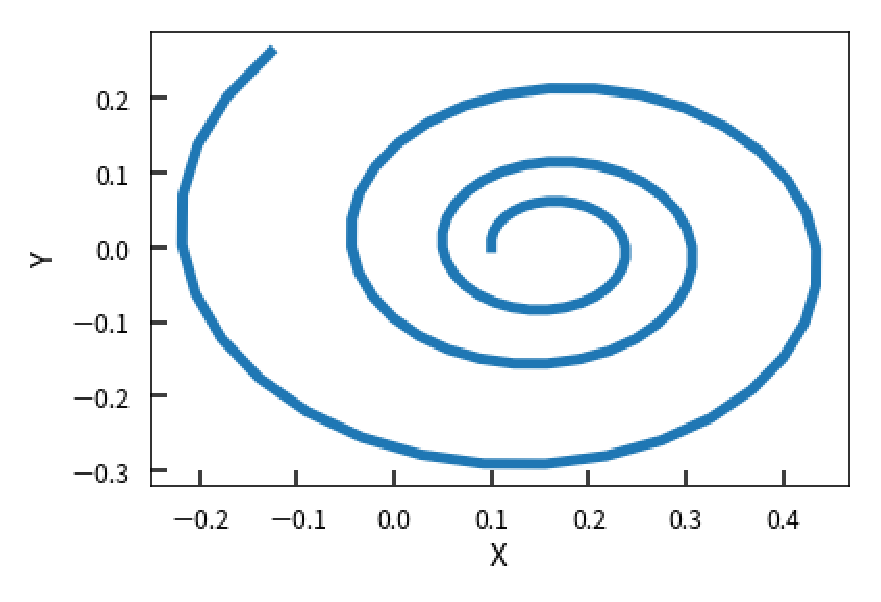
\includegraphics[scale=0.5]{sim9h01xy.eps}
         \end{center}
         \subcaption{位置のグラフ}
         \label{sim9h01xy}
        \end{minipage}

        \begin{minipage}{0.5\hsize}
         \begin{center}
          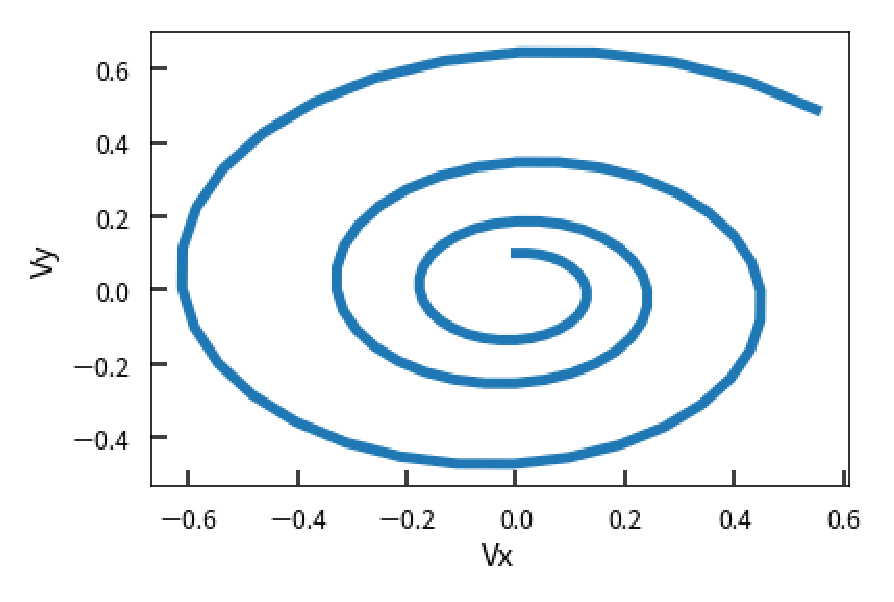
\includegraphics[scale=0.5]{sim9h01vxy.eps}
         \end{center}
         \subcaption{速度のグラフ}
         \label{sim9h01vxy}
        \end{minipage}
      \end{tabular}
        \caption{$h=0.1$のときの実行結果}
        \label{sim9h01}
       \end{figure}
    
       \begin{figure}[H]
        \begin{tabular}{c}
        \begin{minipage}{0.5\hsize}
         \begin{center}
          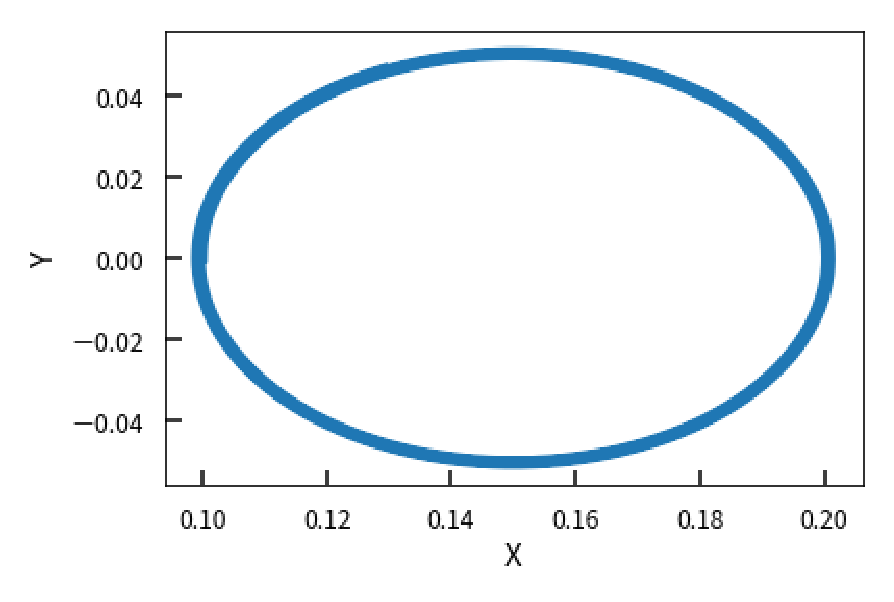
\includegraphics[scale=0.5]{sim9h0001xy.eps}
         \end{center}
         \subcaption{位置のグラフ}
         \label{sim9h0001xy}
        \end{minipage}

        \begin{minipage}{0.5\hsize}
         \begin{center}
          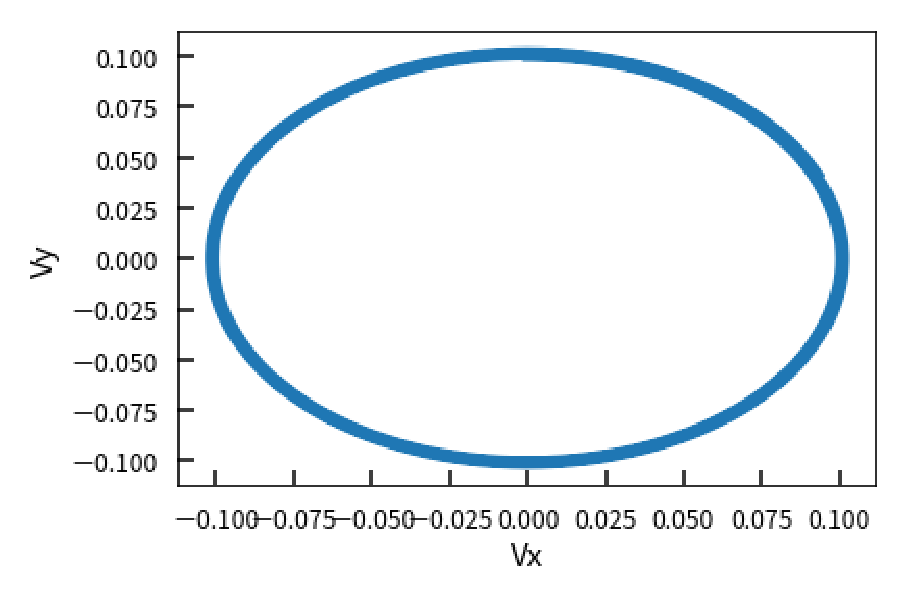
\includegraphics[scale=0.5]{sim9h0001vxy.eps}
         \end{center}
         \subcaption{速度のグラフ}
         \label{sim9h0001vxy}
        \end{minipage}
      \end{tabular}
        \caption{$h=0.001$のときの実行結果}
        \label{sim9h0001}
       \end{figure}

       このように,刻み幅によって,正しい実行結果が得られない場合がある.正しい結果が得られる刻み幅について考察する.
       誤差の測定は,計算値と理論値の$v_x^2+x_y^2$の値を比較することで行う.理論値は$v_x^2+x_y^2=0.01$である.
       表\ref{sim9h8}に刻み幅を変えて,計算を行った結果を示す.表\ref{sim9h8}から,刻み幅を小さくすると誤差が減少し,
       $h=0.001$のとき,誤差の平均が約2\%になることがわかる.このことから刻み幅$h=0.001$を正しい結果が得られる刻み幅と
       考える.

       \begin{table}[H]
        \caption{刻み幅と誤差の関係}
        \label{sim9h8}
        \begin{center}
        \begin{tabular}{r|c|c}\hline
          刻み幅 & 誤差の平均[\%] & 誤差の標準偏差 \\ \hline \hline 
          0.1 & 1262.53 & 1379.76 \\
          0.05 & 232.77 & 185.0 \\
          0.01 & 24.16 & 14.32 \\
          0.005 & 11.25 & 6.42 \\
          0.001 & 2.13 & 1.18 \\ \hline
        \end{tabular}
        \end{center}
        \end{table}

        次に$B_0$を変化させたときの実行結果について確認する.図\ref{B1}~図\ref{B10}に$B_0$を変化させたときの実行結果を
        示す.図\ref{B1}は$B_0=1$,図\ref{B5}は$B_0=5$,図\ref{B10}は$B_0=10$のときの実行結果である.どの結果も0から10秒のとき
        のシミュレーションを行っている.

        \begin{figure}[H]
          \centering
          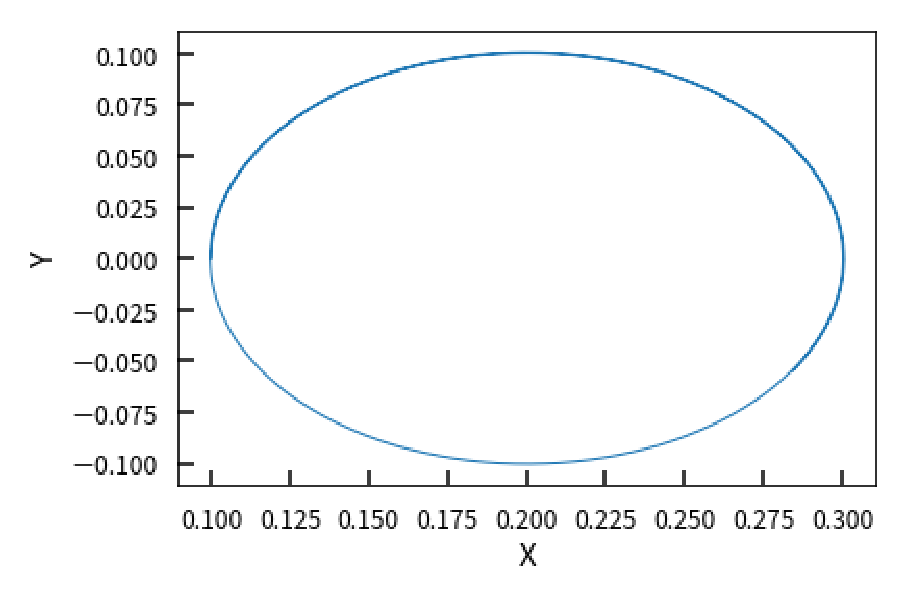
\includegraphics[scale=0.6]{sim9xyB1.eps}
          \caption{$B_0=1$の実行結果}
          \label{B1}
          \end{figure}
          \begin{figure}[H]
            \centering
            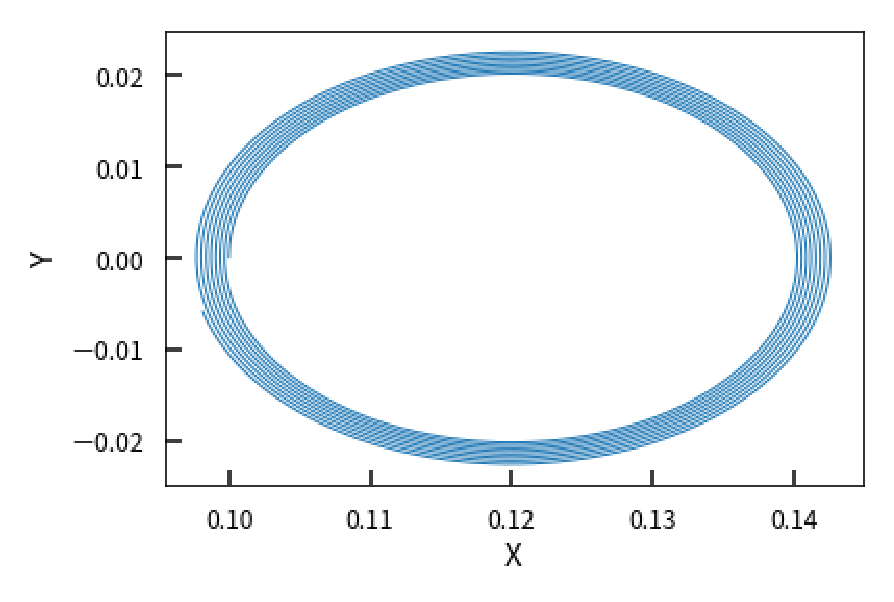
\includegraphics[scale=0.6]{sim9xyB5.eps}
            \caption{$B_0=5$の実行結果}
            \label{B5}
            \end{figure}
        \begin{figure}[H]
          \centering
          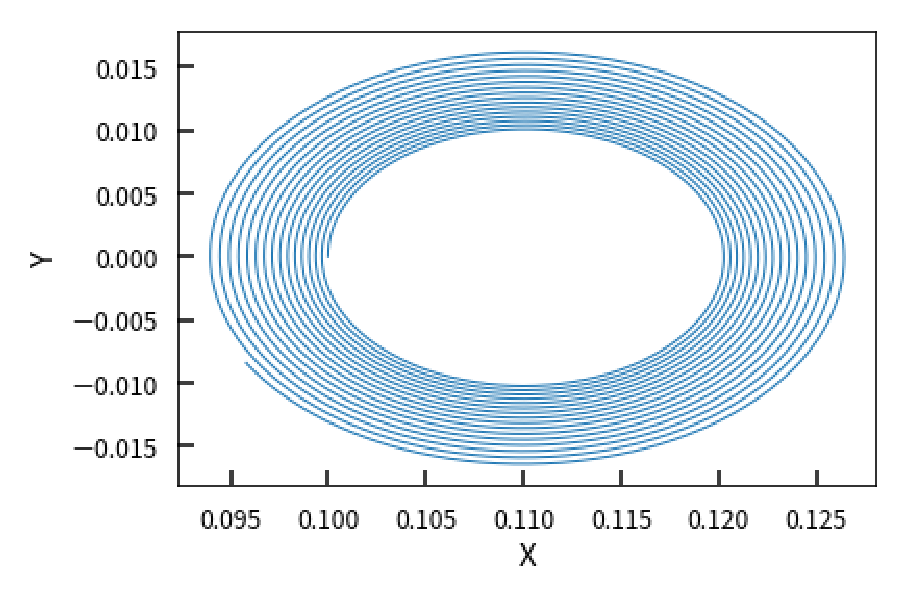
\includegraphics[scale=0.6]{sim9xyB10.eps}
          \caption{$B_0=10$の実行結果}
          \label{B10}
          \end{figure}

          なぜこのようなシミュレーション結果になるのか考察する.速度\mbox{\boldmath $F$}で運動する粒子は一様磁場中で
          円運動をする.円運動の向心力はローレンツ力で,この運動をサイクロトロン運動という.図\ref{B1}~図\ref{B10}から
          円運動の周期は磁場の大きさ$B_0$に依存すると考えられる.このことを確認する.向心力$F=mr \omega^2$およびローレンツ力$f=qvB_0 \sin \theta$
          (磁場と速度は垂直より$\sin \theta =1$)
          より角速度$w$は式(\ref{lorentzomega})で表せる.式(\ref{lorentzomega})から円運動の周期$T$は式(\ref{lorentzt})
          にようになる.いま,電荷$q$,質量$m$は1で固定しているから周期$T$は磁場の大きさ$B_0$のみに依存することがわかる.さらに式(\ref{lorentzt})から
          磁場の大きさ$B_0$が小さいとき,周期が長くなり, 磁場の大きさ$B_0$が大きいとき,周期が短くなる関係があることが読み取れる.図\ref{B1}~図\ref{B10}
          からもこの関係が読み取れる. $B_0=1$(図\ref{B1})のときは,同じ時間あたりの回転数が少なく, $B_0=10$(図\ref{B1})のときは$B_0=1$と比較して
          回転数が多い.これらの考察から,円運動をするというシミュレーション結果が正しいと考察する.


          \begin{eqnarray}
            mr \omega^2 &=& qvB_0 \\
            \omega &=& \frac{q}{m}B_0 \label{lorentzomega} \\
            T &=& \frac{2 \pi}{\omega} \\
            T &=& 2 \pi \sqrt{\frac{m}{qB_0}} \label{lorentzt}
          \end{eqnarray}             


      \subsubsection{課題10の実行結果と考察}
        図\ref{b2e1}~図\ref{b05e1xyz}にリスト\ref{kadai10}のコードの実行結果を示す.
        図\ref{b2e1}および図\ref{b2e1xyz}は$E=1.0$かつ$B=2.0$のときの実行結果,
        図\ref{b05e1}および図\ref{b05e1xyz}は$E=1.0$かつ$B=0.5$のときの実行結果である.
        図\ref{b2e1}~図\ref{b05e1xyz}から,電場$E$が加わると,xy方向は円運動,z方向は上昇する運動をすることが
        読み取れる.

        \begin{figure}[H]
          \centering
          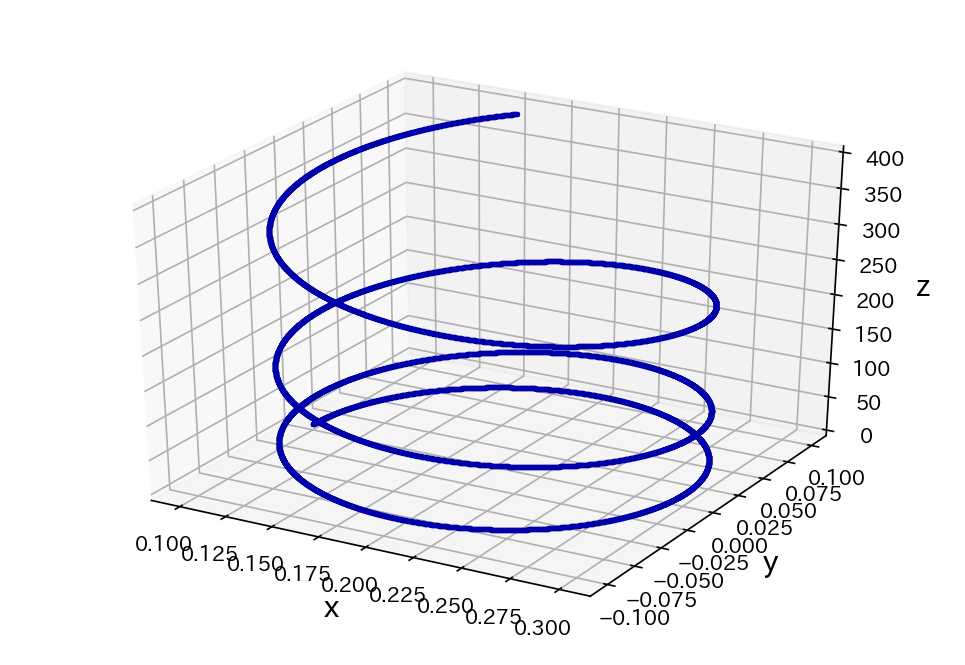
\includegraphics[scale=0.6]{b2e1.eps}
          \caption{$E=1.0$かつ$B=2.0$のときの実行結果(3D)}
          \label{b2e1}
          \end{figure}

        \begin{figure}[H]
          \centering
          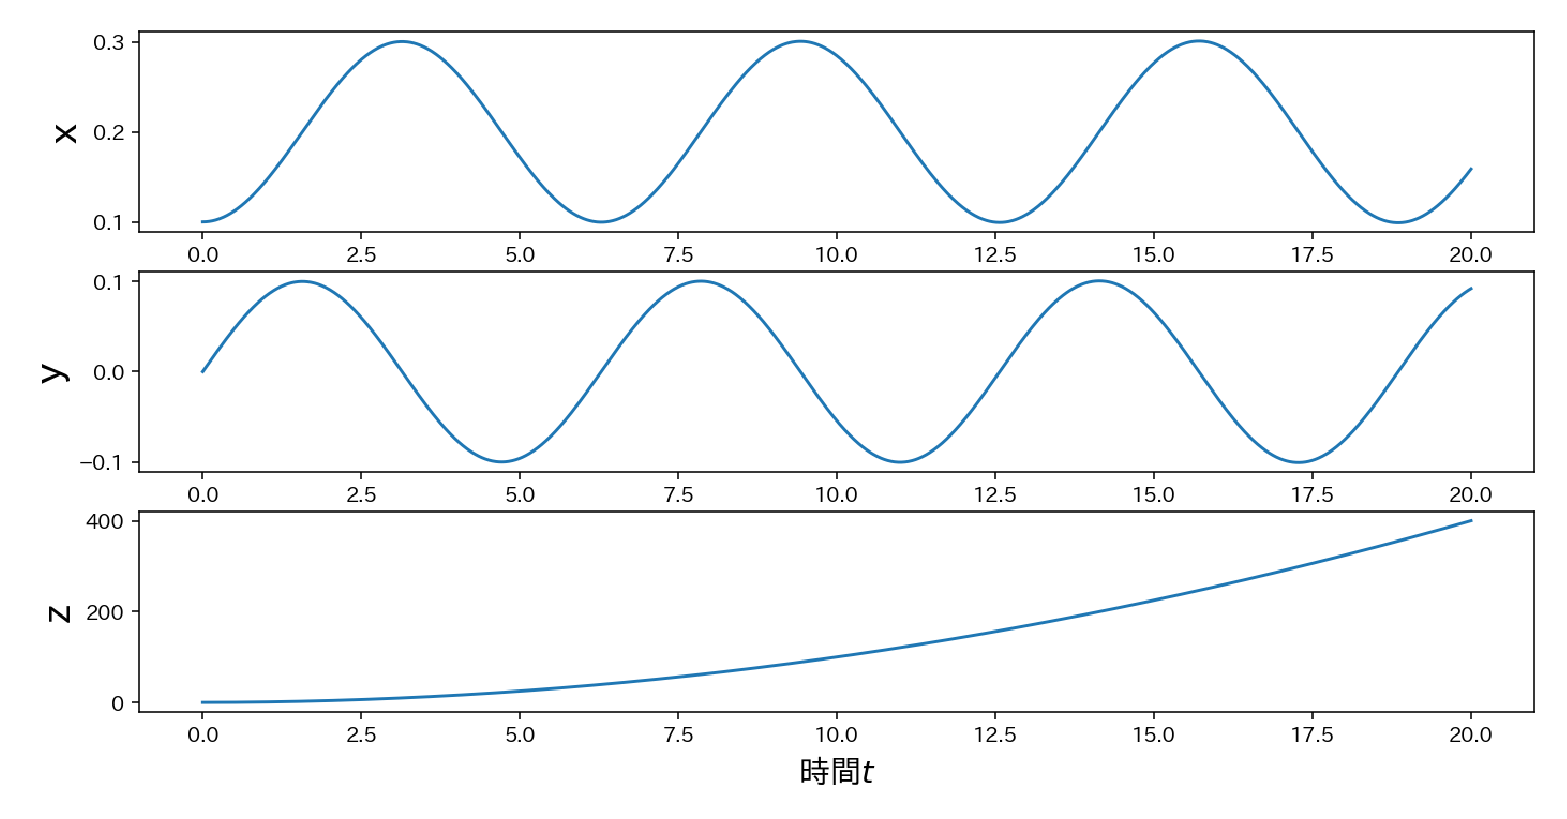
\includegraphics[scale=0.5]{b2e1xyz.eps}
          \caption{$E=1.0$かつ$B=2.0$のときの実行結果(成分ごと)}
          \label{b2e1xyz}
          \end{figure}

        \begin{figure}[H]
          \centering
          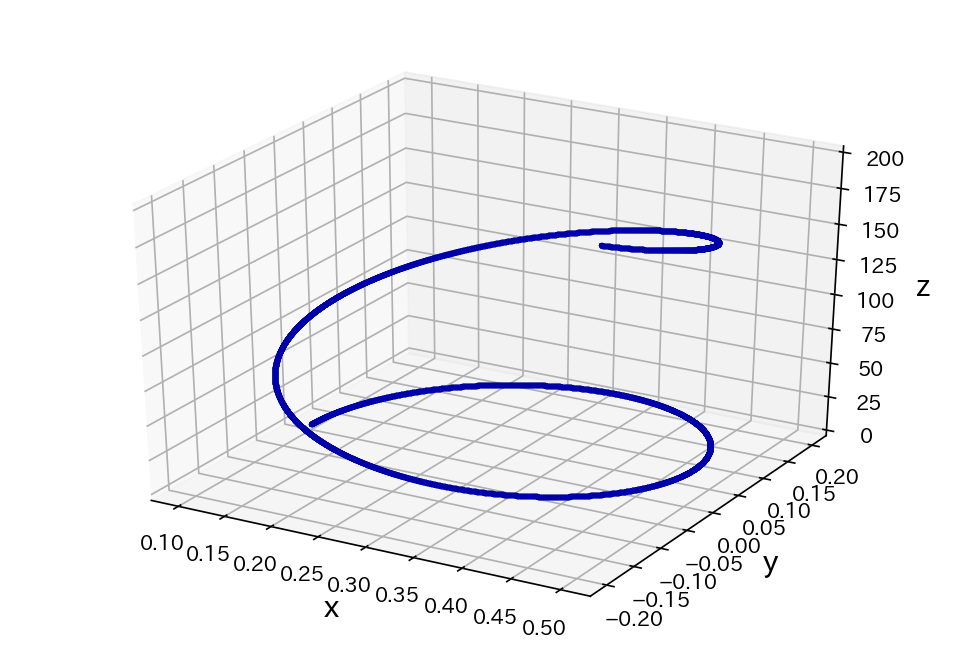
\includegraphics[scale=0.6]{b05e1.eps}
          \caption{$E=1.0$かつ$B=0.5$のときの実行結果(3D)}
          \label{b05e1}
          \end{figure}

        \begin{figure}[H]
          \centering
          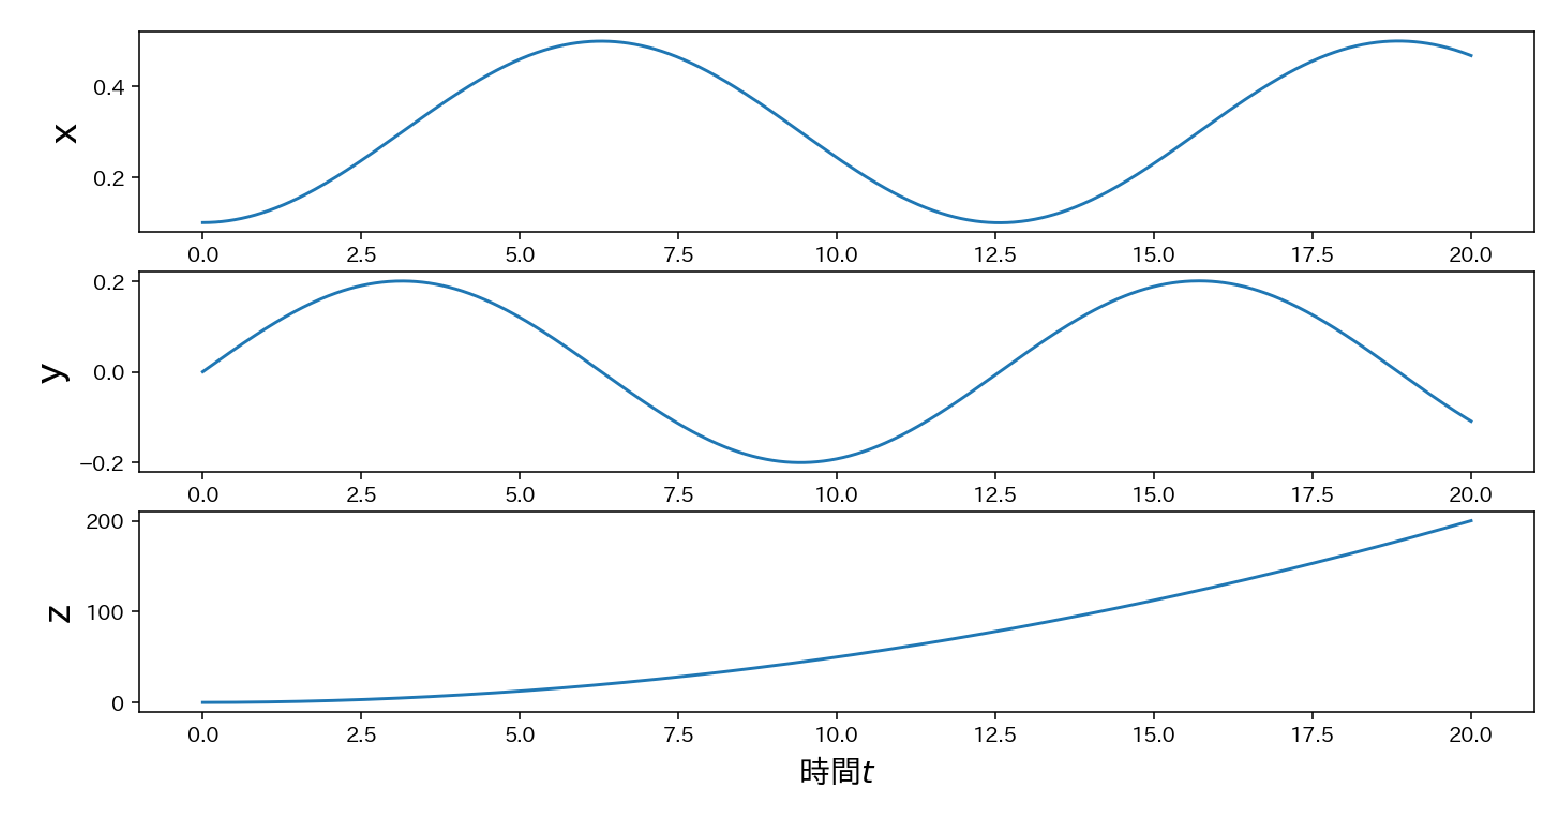
\includegraphics[scale=0.5]{b05e1xyz.eps}
          \caption{$E=1.0$かつ$B=0.5$のときの実行結果(成分ごと)}
          \label{b05e1xyz}
          \end{figure}

          z方向の運動について考察する.式(\ref{ef})からz方向の運動は簡単に解くことができる.
          式(\ref{zz})に式(\ref{ef})からz方向の運動を解いたときの結果を示す.
          式(\ref{ef})からz方向の運動は二次関数であることがわかる.シミュレーション結果(図\ref{b2e1}~図\ref{b05e1xyz})
          を確認すると,z方向の運動は確かに二次関数であることがわかる.理論値と計算値が一致していることも確認する.
          図\ref{b05e1th}に式(\ref{ef})から$E=1.0$かつ$B=0.5$のときの,z方向の理論値を計算してプロットしたグラフを示す.
          図\ref{b05e1th}から理論値と計算値は目視ではすべて一致していることが読み取れる.

          \begin{eqnarray}
              \frac{dv_z}{dt} = \frac{q}{m}E_z \\
              v_z = \frac{q}{m}E_z t \\
              Z = \frac{q E_z}{2m}t^2 \label{zz}
          \end{eqnarray}

          \begin{figure}[H]
            \centering
            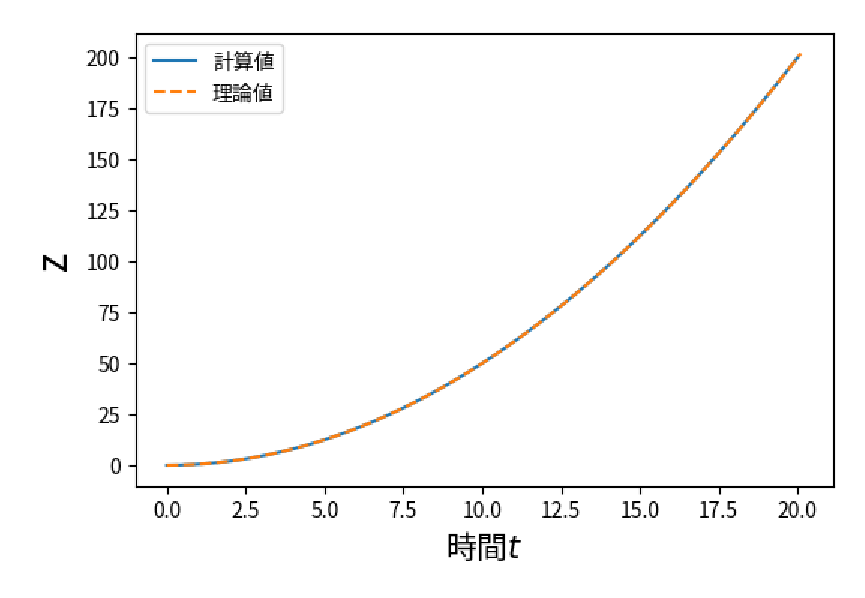
\includegraphics[scale=0.7]{b05e1th.eps}
            \caption{理論値と計算値が一致することの確認}
            \label{b05e1th}
            \end{figure}

        \begin{thebibliography}{9}
          \bibitem{cu} 服部 憲司,"例題と演習で学ぶ 続・電気回路",森北出版株式会社,2017 
          \end{thebibliography}
\end{document}

